% Project Technical Documentation
\documentclass[12pt,a4paper]{article}
\usepackage[utf8]{inputenc}
\usepackage{graphicx}
\usepackage{listings}
\usepackage{xcolor}
\usepackage{hyperref}
\usepackage{tikz}

\usepackage{pgf-umlsd}
\usepackage{amsmath}
\usepackage{float}
\usepackage{array}
\usepackage{booktabs}
\usepackage{longtable}
\usepackage{tabularx}
\usepackage{multicol}
\usepackage{enumitem}
\usepackage[most]{tcolorbox}
\usetikzlibrary{positioning,shapes,arrows,fit,calc,graphs,graphs.standard}

% Define colors for different elements
\definecolor{codegreen}{rgb}{0,0.6,0}
\definecolor{codegray}{rgb}{0.5,0.5,0.5}
\definecolor{codepurple}{rgb}{0.58,0,0.82}
\definecolor{backcolour}{rgb}{0.95,0.95,0.92}

% Configure code listings
\lstdefinestyle{mystyle}{
    backgroundcolor=\color{backcolour},   
    commentstyle=\color{codegreen},
    keywordstyle=\color{magenta},
    numberstyle=\tiny\color{codegray},
    stringstyle=\color{codepurple},
    basicstyle=\ttfamily\small,
    breakatwhitespace=false,         
    breaklines=true,                 
    captionpos=b,                    
    keepspaces=true,                 
    numbers=left,                    
    numbersep=5pt,                  
    showspaces=false,                
    showstringspaces=false,
    showtabs=false,                  
    tabsize=2
}
\lstset{style=mystyle}

% Define custom boxes for important information
\newtcolorbox{infobox}[1]{colback=blue!5!white,colframe=blue!75!black,title=#1}
\newtcolorbox{warningbox}[1]{colback=orange!5!white,colframe=orange!75!black,title=#1}
\newtcolorbox{tipbox}[1]{colback=green!5!white,colframe=green!75!black,title=#1}

\title{\Huge{\textbf{Technical Documentation:}}\\ \huge{Placement Management System}\\ \Large{Comprehensive Analysis and Architecture Documentation}}
\author{Project Team}
\date{\today}

\begin{document}

\maketitle
\tableofcontents
\newpage

\section{Introduction}
\begin{multicols}{2}
This document provides a comprehensive technical overview of our Placement Management System, which is built using React.js for the frontend and Node.js for the backend. The application implements a modern architecture with various features including user authentication, data visualization, and real-time communication capabilities specifically designed for managing campus placements.

The system is designed to provide a scalable, maintainable, and robust platform for handling student placement activities, company recruitment processes, and administrative workflows while delivering an intuitive and responsive user experience. This documentation covers the architectural decisions, technology choices, implementation details, and development practices employed throughout the project.

\begin{infobox}{Project Goals}
\begin{itemize}
    \item Create a responsive platform for students, companies, and placement officers
    \item Implement secure authentication and role-based authorization
    \item Enable real-time placement analytics and reporting
    \item Ensure scalability to handle peak recruitment seasons
    \item Maintain code quality and long-term maintainability
    \item Provide comprehensive documentation for future enhancement
\end{itemize}
\end{infobox}
\end{multicols}

\subsection{Project Background}
The Placement Management System was developed to address the growing need for a centralized platform that streamlines the campus recruitment process. Traditional placement management often involves manual processes, fragmented communication, and limited analytics capabilities, creating inefficiencies for all stakeholders.

By leveraging modern web technologies, we've created a comprehensive solution that bridges these gaps while providing a foundation for future enhancements and integrations with other campus systems like student information systems and learning management platforms.

\subsection{Target Audience}
The system serves multiple user roles including:
\begin{itemize}
    \item Students seeking placement opportunities and tracking applications
    \item Company recruiters posting positions and managing candidates
    \item Placement officers coordinating recruitment activities
    \item University administrators accessing analytics and reports
    \item System administrators maintaining the platform
\end{itemize}

\section{System Architecture}

\subsection{High-Level Architecture}
The Placement Management System follows a modern client-server architecture with clearly separated frontend and backend components. This separation allows for independent scaling, maintenance, and deployment of each component while ensuring clean interface contracts between layers.

\begin{figure}[H]
\centering
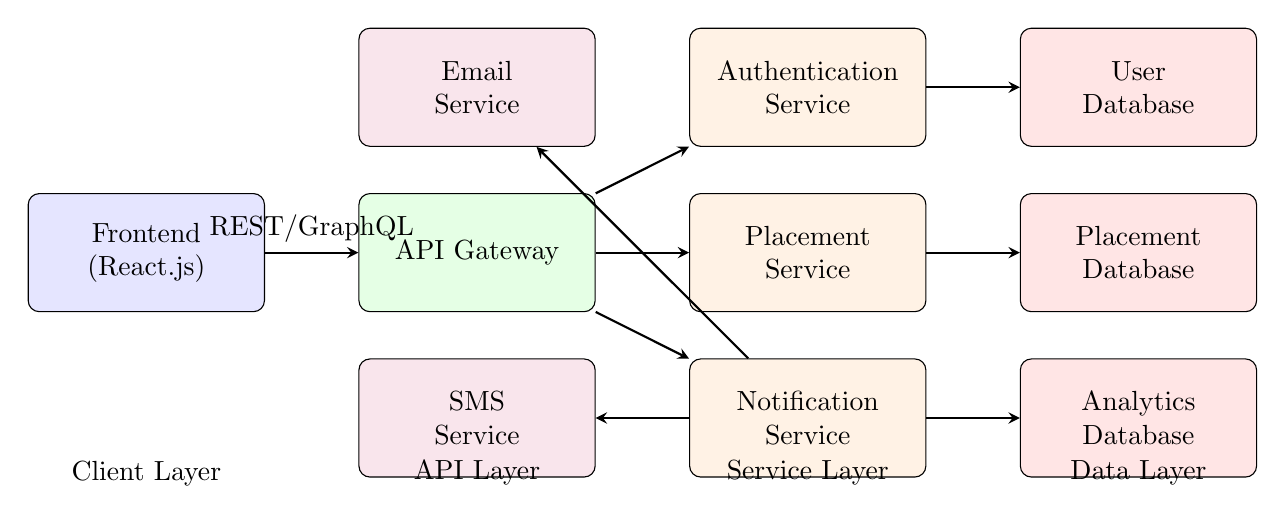
\begin{tikzpicture}[scale=0.7, 
    box/.style={draw, minimum width=3cm, minimum height=1.5cm, align=center, rounded corners},
    arrow/.style={->, >=stealth, thick}]
    
    % Frontend
    \node[box, fill=blue!10] (frontend) at (0,0) {Frontend\\(React.js)};
    
    % API Gateway
    \node[box, fill=green!10] (api) at (6,0) {API Gateway};
    
    % Backend Services
    \node[box, fill=orange!10] (auth) at (12,3) {Authentication\\Service};
    \node[box, fill=orange!10] (data) at (12,0) {Placement\\Service};
    \node[box, fill=orange!10] (notify) at (12,-3) {Notification\\Service};
    
    % Databases
    \node[box, fill=red!10] (authdb) at (18,3) {User\\Database};
    \node[box, fill=red!10] (maindb) at (18,0) {Placement\\Database};
    \node[box, fill=red!10] (logdb) at (18,-3) {Analytics\\Database};
    
    % External Services
    \node[box, fill=purple!10] (email) at (6,3) {Email\\Service};
    \node[box, fill=purple!10] (sms) at (6,-3) {SMS\\Service};
    
    % Connect components with arrows
    \draw[arrow] (frontend) -- (api) node[midway, above] {REST/GraphQL};
    \draw[arrow] (api) -- (auth);
    \draw[arrow] (api) -- (data);
    \draw[arrow] (api) -- (notify);
    \draw[arrow] (auth) -- (authdb);
    \draw[arrow] (data) -- (maindb);
    \draw[arrow] (notify) -- (logdb);
    \draw[arrow] (notify) -- (email);
    \draw[arrow] (notify) -- (sms);
    
    % Labels
    \node[align=center] at (0,-4) {Client Layer};
    \node[align=center] at (6,-4) {API Layer};
    \node[align=center] at (12,-4) {Service Layer};
    \node[align=center] at (18,-4) {Data Layer};
\end{tikzpicture}
\caption{Detailed System Architecture Overview}
\end{figure}

\subsection{Architectural Patterns}
The system incorporates several architectural patterns to address different aspects of the application:

\begin{itemize}
    \item \textbf{Microservices Architecture}: Backend functionality is divided into distinct services that can be developed, deployed, and scaled independently.
    
    \item \textbf{Model-View-Controller (MVC)}: The frontend implements a variation of MVC pattern where React components serve as views, custom hooks handle control logic, and data models are maintained in state management systems.
    
    \item \textbf{Repository Pattern}: Data access is abstracted through repository interfaces to decouple business logic from data storage mechanisms.
    
    \item \textbf{Command Query Responsibility Segregation (CQRS)}: Operations that modify data (commands) are separated from operations that read data (queries) to optimize performance and scalability.
    
    \item \textbf{Event-Driven Architecture}: System components communicate asynchronously through events, allowing for loose coupling and better fault tolerance.
\end{itemize}

\subsection{Communication Flow}
\begin{figure}[H]
\centering
\begin{tikzpicture}[scale=0.65, node distance=2.5cm,
    process/.style={rectangle, draw, minimum width=2cm, minimum height=1cm, align=center, rounded corners},
    data/.style={cylinder, draw, shape aspect=0.3, minimum width=2cm, minimum height=1cm, align=center},
    arrow/.style={->, >=stealth, thick}]
    
    % User types
    \node[process] (student) {Student};
    \node[process, right=of student] (company) {Company};
    \node[process, right=of company] (admin) {Placement Officer};
    
    % UI Components
    \node[process, below=of student, xshift=2.5cm] (ui) {UI Components};
    
    % State Management
    \node[process, below=of ui] (state) {State Management};
    
    % API Service
    \node[process, below=of state] (api) {API Service};
    
    % Backend Controller
    \node[process, below=of api] (controller) {Backend Controller};
    
    % Service Layer
    \node[process, below=of controller] (service) {Service Layer};
    
    % Data Access
    \node[process, below=of service] (data) {Data Access Layer};
    
    % Database
    \node[data, below=of data] (db) {Database};
    
    % Connect with arrows
    \draw[arrow] (student) -- (ui);
    \draw[arrow] (company) -- (ui);
    \draw[arrow] (admin) -- (ui);
    \draw[arrow] (ui) -- (state) node[midway, right] {State Updates};
    \draw[arrow] (state) -- (api) node[midway, right] {API Calls};
    \draw[arrow] (api) -- (controller) node[midway, right] {HTTP Requests};
    \draw[arrow] (controller) -- (service) node[midway, right] {Business Logic};
    \draw[arrow] (service) -- (data) node[midway, right] {Data Operations};
    \draw[arrow] (data) -- (db) node[midway, right] {CRUD Operations};
    
    % Response path - use a different route to avoid overlapping
    \draw[arrow, dashed] (db) -- +(-4,0) |- (data);
    \draw[arrow, dashed] (data) -- +(-4,0) |- (service);
    \draw[arrow, dashed] (service) -- +(-4,0) |- (controller);
    \draw[arrow, dashed] (controller) -- +(-4,0) |- (api);
    \draw[arrow, dashed] (api) -- +(-4,0) |- (state);
    \draw[arrow, dashed] (state) -- +(-4,0) |- (ui);
    \draw[arrow, dashed] (ui.west) -| (student);
    \draw[arrow, dashed] (ui) -- (company);
    \draw[arrow, dashed] (ui.east) -| (admin);
    
    \node[right] at (-6, -9) {Response Flow};
    \node[right] at (4, -9) {Request Flow};
\end{tikzpicture}
\caption{Placement Management System Communication Flow}
\end{figure}

\section{Technology Stack}

The application leverages a modern technology stack designed to provide optimal performance, maintainability, and developer experience. Each technology was carefully selected based on its strengths, community support, and alignment with project requirements.

\begin{figure}[H]
\centering
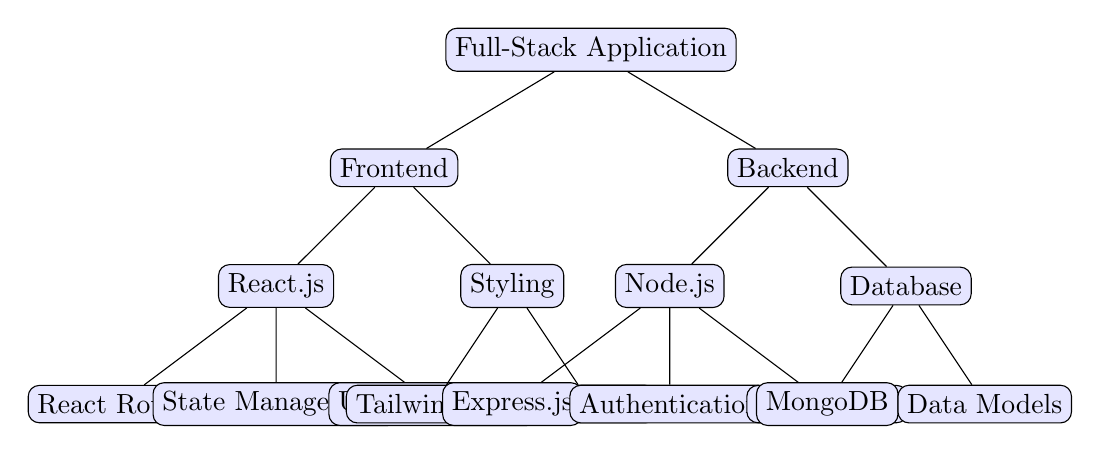
\begin{tikzpicture}[
  level 1/.style={sibling distance=50mm},
  level 2/.style={sibling distance=30mm},
  level 3/.style={sibling distance=20mm},
  every node/.style={shape=rectangle, rounded corners, draw, align=center, fill=blue!10}
]
  % Root
  \node{Full-Stack Application}
    % Main branches
    child {node{Frontend}
      child {node{React.js}
        child {node{React Router}}
        child {node{State Management}}
        child {node{UI Components}}
      }
      child {node{Styling}
        child {node{TailwindCSS}}
        child {node{Radix UI}}
      }
    }
    child {node{Backend}
      child {node{Node.js}
        child {node{Express.js}}
        child {node{Authentication}}
        child {node{API Routes}}
      }
      child {node{Database}
        child {node{MongoDB}}
        child {node{Data Models}}
      }
    };
\end{tikzpicture}
\caption{Technology Stack Overview}
\end{figure}

\subsection{Frontend Technologies}
\begin{multicols}{2}
\begin{itemize}
    \item \textbf{React.js (v19.0.0)}
    \begin{itemize}
        \item Component-based UI architecture
        \item Virtual DOM for efficient rendering
        \item Hooks for state management and side effects
        \item Context API for global state sharing
    \end{itemize}
    
    \item \textbf{React Router DOM (v7.1.5)}
    \begin{itemize}
        \item Client-side routing with history management
        \item Lazy loading for code splitting
        \item Route-based code splitting
        \item Protected route implementation
    \end{itemize}
    
    \item \textbf{TailwindCSS (v3.4.17)}
    \begin{itemize}
        \item Utility-first CSS framework
        \item JIT (Just-In-Time) compilation
        \item Responsive design utilities
        \item Custom design system implementation
    \end{itemize}
    
    \item \textbf{Radix UI Components}
    \begin{itemize}
        \item Accessible component primitives
        \item Unstyled components with full styling control
        \item Focus management and keyboard navigation
        \item Screen reader compatibility
    \end{itemize}
    
    \item \textbf{Recharts for Data Visualization}
    \begin{itemize}
        \item Chart components built with D3
        \item Responsive and interactive visualizations
        \item Customizable chart elements
        \item Support for various chart types
    \end{itemize}
    
    \item \textbf{Axios for HTTP Requests}
    \begin{itemize}
        \item Promise-based HTTP client
        \item Request/response interceptors
        \item Automatic JSON parsing
        \item Request cancellation support
    \end{itemize}
\end{itemize}
\end{multicols}

\begin{figure}[H]
\centering
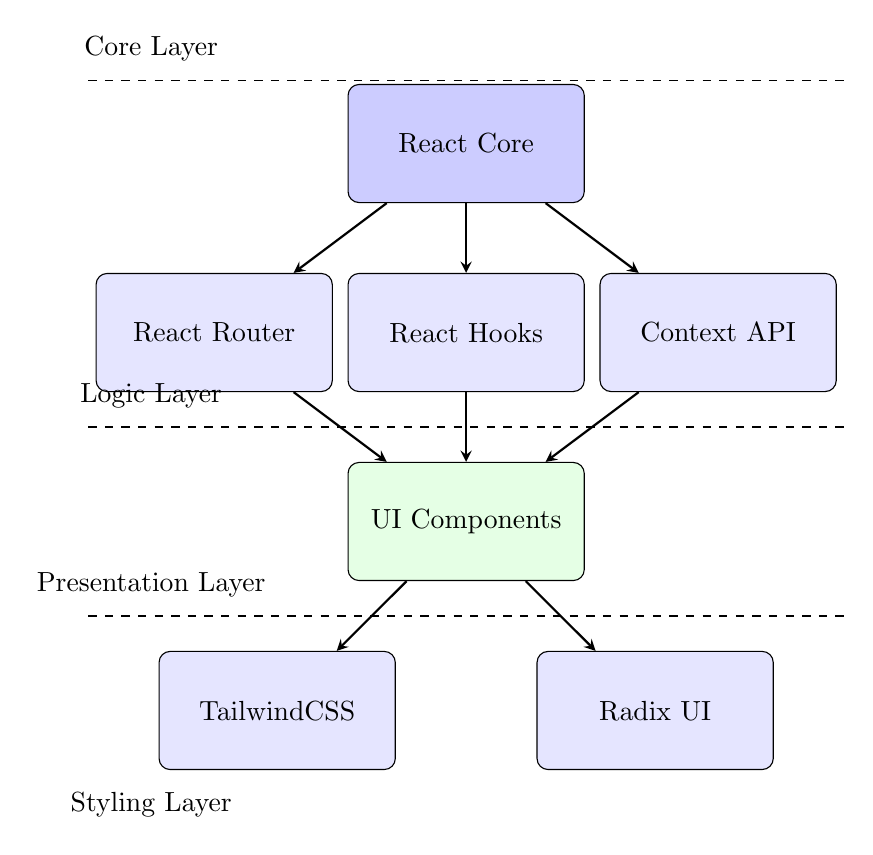
\begin{tikzpicture}[scale=0.8, 
    block/.style={rectangle, draw, minimum width=3cm, minimum height=1.5cm, align=center, rounded corners, fill=blue!10},
    arrow/.style={->, >=stealth, thick}]
    
    % React Core
    \node[block, fill=blue!20] (react) at (0,0) {React Core};
    
    % Connected components
    \node[block] (router) at (-4,-3) {React Router};
    \node[block] (hooks) at (0,-3) {React Hooks};
    \node[block] (context) at (4,-3) {Context API};
    
    % UI Layer
    \node[block, fill=green!10] (components) at (0,-6) {UI Components};
    
    % Styling
    \node[block] (tailwind) at (-3,-9) {TailwindCSS};
    \node[block] (radix) at (3,-9) {Radix UI};
    
    % Connect components
    \draw[arrow] (react) -- (router);
    \draw[arrow] (react) -- (hooks);
    \draw[arrow] (react) -- (context);
    \draw[arrow] (router) -- (components);
    \draw[arrow] (hooks) -- (components);
    \draw[arrow] (context) -- (components);
    \draw[arrow] (components) -- (tailwind);
    \draw[arrow] (components) -- (radix);
    
    % Layers
    \draw[dashed] (-6,1) -- (6,1);
    \node at (-5,1.5) {Core Layer};
    
    \draw[dashed] (-6,-4.5) -- (6,-4.5);
    \node at (-5,-4) {Logic Layer};
    
    \draw[dashed] (-6,-7.5) -- (6,-7.5);
    \node at (-5,-7) {Presentation Layer};
    
    \node at (-5,-10.5) {Styling Layer};
\end{tikzpicture}
\caption{Frontend Architecture Layers}
\end{figure}

\subsection{Backend Technologies}
\begin{multicols}{2}
\begin{itemize}
    \item \textbf{Node.js}
    \begin{itemize}
        \item Event-driven, non-blocking I/O
        \item JavaScript runtime environment
        \item V8 JavaScript engine
        \item Support for ES6+ features
    \end{itemize}
    
    \item \textbf{Express.js}
    \begin{itemize}
        \item Minimal web application framework
        \item Middleware-based request pipeline
        \item Routing system with parameter support
        \item Template engine integration
    \end{itemize}
    
    \item \textbf{MongoDB}
    \begin{itemize}
        \item NoSQL document database
        \item Flexible schema design
        \item Horizontal scaling capabilities
        \item Native JSON document support
    \end{itemize}
    
    \item \textbf{Mongoose ODM}
    \begin{itemize}
        \item MongoDB object modeling
        \item Schema validation
        \item Middleware hooks
        \item Query building API
    \end{itemize}
    
    \item \textbf{Nodemailer for Email Services}
    \begin{itemize}
        \item SMTP transport
        \item HTML email support
        \item Attachment handling
        \item Email template support
    \end{itemize}
    
    \item \textbf{Twilio for SMS Services}
    \begin{itemize}
        \item SMS messaging
        \item MMS capabilities
        \item Phone number verification
        \item Two-factor authentication
    \end{itemize}
    
    \item \textbf{JWT for Authentication}
    \begin{itemize}
        \item Stateless authentication
        \item Token-based access control
        \item Expiration and refresh mechanisms
        \item Signature verification
    \end{itemize}
\end{itemize}
\end{multicols}

\begin{figure}[H]
\centering
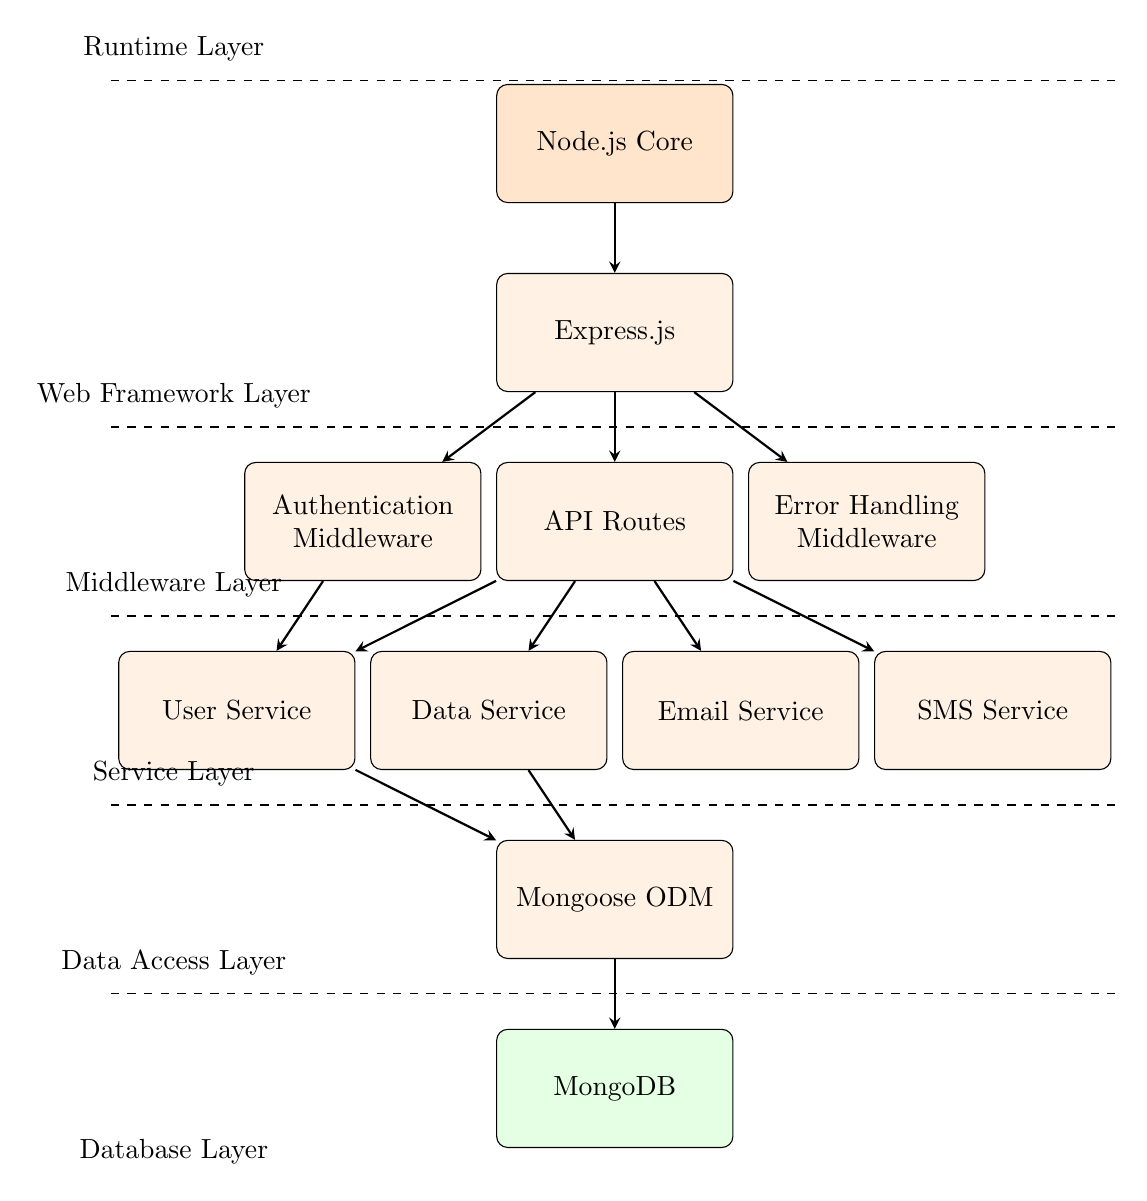
\begin{tikzpicture}[scale=0.8, 
    block/.style={rectangle, draw, minimum width=3cm, minimum height=1.5cm, align=center, rounded corners, fill=orange!10},
    arrow/.style={->, >=stealth, thick}]
    
    % Node.js Core
    \node[block, fill=orange!20] (node) at (0,0) {Node.js Core};
    
    % Main components
    \node[block] (express) at (0,-3) {Express.js};
    
    % Middleware layer
    \node[block] (auth) at (-4,-6) {Authentication\\Middleware};
    \node[block] (routes) at (0,-6) {API Routes};
    \node[block] (error) at (4,-6) {Error Handling\\Middleware};
    
    % Service layer
    \node[block] (user) at (-6,-9) {User Service};
    \node[block] (data) at (-2,-9) {Data Service};
    \node[block] (email) at (2,-9) {Email Service};
    \node[block] (sms) at (6,-9) {SMS Service};
    
    % Data access layer
    \node[block] (mongoose) at (0,-12) {Mongoose ODM};
    
    % Database
    \node[block, fill=green!10] (mongodb) at (0,-15) {MongoDB};
    
    % Connect components
    \draw[arrow] (node) -- (express);
    \draw[arrow] (express) -- (auth);
    \draw[arrow] (express) -- (routes);
    \draw[arrow] (express) -- (error);
    \draw[arrow] (auth) -- (user);
    \draw[arrow] (routes) -- (user);
    \draw[arrow] (routes) -- (data);
    \draw[arrow] (routes) -- (email);
    \draw[arrow] (routes) -- (sms);
    \draw[arrow] (user) -- (mongoose);
    \draw[arrow] (data) -- (mongoose);
    \draw[arrow] (mongoose) -- (mongodb);
    
    % Layers
    \draw[dashed] (-8,1) -- (8,1);
    \node at (-7,1.5) {Runtime Layer};
    
    \draw[dashed] (-8,-4.5) -- (8,-4.5);
    \node at (-7,-4) {Web Framework Layer};
    
    \draw[dashed] (-8,-7.5) -- (8,-7.5);
    \node at (-7,-7) {Middleware Layer};
    
    \draw[dashed] (-8,-10.5) -- (8,-10.5);
    \node at (-7,-10) {Service Layer};
    
    \draw[dashed] (-8,-13.5) -- (8,-13.5);
    \node at (-7,-13) {Data Access Layer};
    
    \node at (-7,-16) {Database Layer};
\end{tikzpicture}
\caption{Backend Architecture Layers}
\end{figure}

\section{Project Structure}

\subsection{Frontend Structure}
The frontend follows a component-based architecture with a structured folder organization to ensure scalability and maintainability. The structure is designed to promote reusability, separation of concerns, and easy navigation for developers.

\begin{figure}[H]
\centering
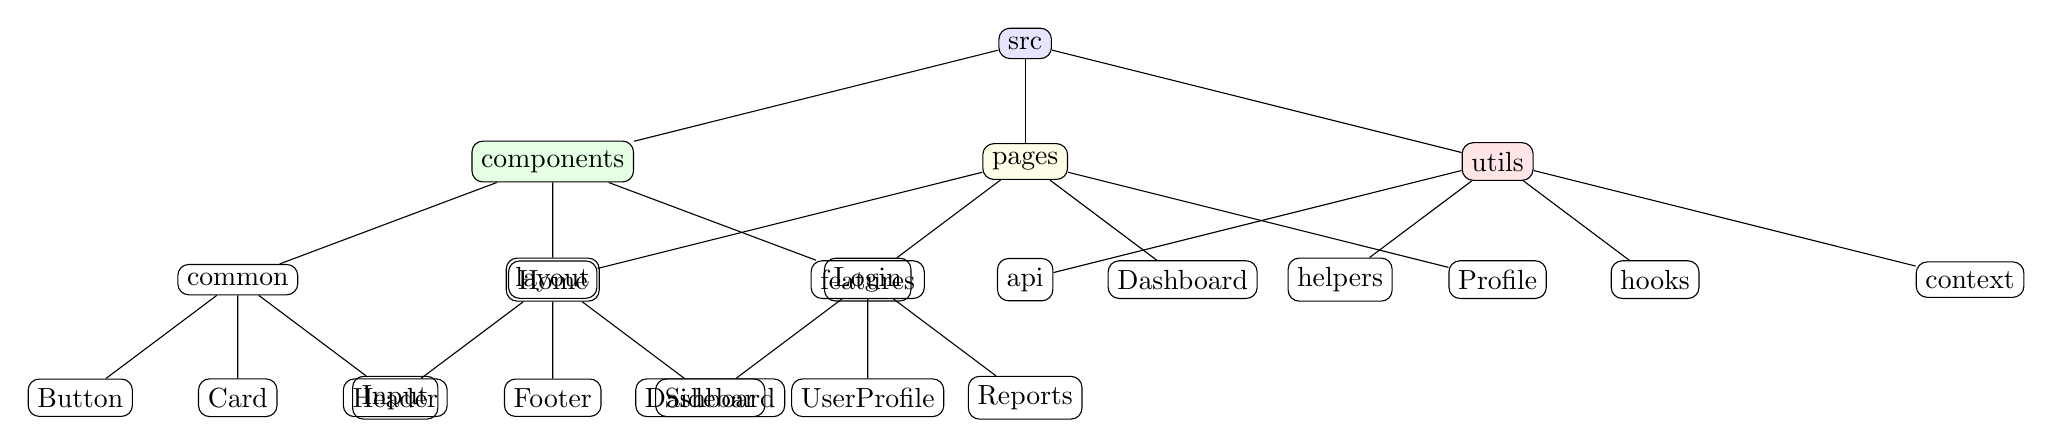
\begin{tikzpicture}[
    every node/.style={rectangle, draw, rounded corners, align=center},
    level 1/.style={sibling distance=6cm},
    level 2/.style={sibling distance=4cm},
    level 3/.style={sibling distance=2cm},
    level distance=1.5cm
]
\node[fill=blue!10] {src}
    child {node[fill=green!10] {components}
        child {node {common}
            child {node {Button}}
            child {node {Card}}
            child {node {Input}}
        }
        child {node {layout}
            child {node {Header}}
            child {node {Footer}}
            child {node {Sidebar}}
        }
        child {node {features}
            child {node {Dashboard}}
            child {node {UserProfile}}
            child {node {Reports}}
        }
    }
    child {node[fill=yellow!10] {pages}
        child {node {Home}}
        child {node {Login}}
        child {node {Dashboard}}
        child {node {Profile}}
    }
    child {node[fill=red!10] {utils}
        child {node {api}}
        child {node {helpers}}
        child {node {hooks}}
        child {node {context}}
    };
\end{tikzpicture}
\caption{Frontend Directory Structure}
\end{figure}

The frontend follows a structured organization with the following key directories:

\begin{lstlisting}[language=bash]
src/
├── components/     # Reusable UI components
│   ├── common/     # Shared basic components
│   ├── layout/     # Page layout components
│   └── features/   # Feature-specific components
├── pages/          # Page components and routes
├── utils/          # Utility functions and helpers
│   ├── api/        # API service functions
│   ├── hooks/      # Custom React hooks
│   └── context/    # Context providers
├── assets/         # Static assets and resources
├── styles/         # Global styles and themes
├── App.js          # Main application component
└── index.js        # Application entry point
\end{lstlisting}

\subsubsection{Component Structure}
Each component follows a consistent structure to promote readability and maintainability:

\begin{lstlisting}[language=JavaScript]
// ComponentName.js - Main component file
import React from 'react';
import PropTypes from 'prop-types';
import './ComponentName.css'; // Scoped styles
import { useComponentLogic } from './useComponentLogic'; // Custom hook

const ComponentName = ({ prop1, prop2, children }) => {
  const { state, handlers } = useComponentLogic(prop1, prop2);
  
  return (
    <div className="component-container">
      {/* Component JSX structure */}
    </div>
  );
};

ComponentName.propTypes = {
  prop1: PropTypes.string.isRequired,
  prop2: PropTypes.number,
  children: PropTypes.node
};

export default ComponentName;
\end{lstlisting}

\begin{lstlisting}[language=JavaScript]
// useComponentLogic.js - Separated business logic
import { useState, useEffect, useCallback } from 'react';

export const useComponentLogic = (prop1, prop2) => {
  const [state, setState] = useState(initialState);
  
  useEffect(() => {
    // Side effects
  }, [dependencies]);
  
  const handleEvent = useCallback(() => {
    // Event handling logic
  }, [dependencies]);
  
  return {
    state,
    handlers: {
      handleEvent
    }
  };
};
\end{lstlisting}

\subsubsection{Page Structure}
Pages follow a similar pattern but include routing and layout considerations:

\begin{lstlisting}[language=JavaScript]
// PageName.js
import React from 'react';
import { MainLayout } from '../components/layout';
import { ComponentA, ComponentB } from '../components/features';
import { usePageLogic } from './usePageLogic';

const PageName = () => {
  const { data, loading, error, actions } = usePageLogic();
  
  if (loading) return <LoadingIndicator />;
  if (error) return <ErrorDisplay message={error} />;
  
  return (
    <MainLayout>
      <PageHeader title="Page Title" />
      <ComponentA data={data.partA} onAction={actions.handleActionA} />
      <ComponentB data={data.partB} onAction={actions.handleActionB} />
    </MainLayout>
  );
};

export default PageName;
\end{lstlisting}

\subsection{Backend Structure}
The backend implements a modular architecture with clear separation of concerns following the principles of clean architecture. The structure facilitates testing, maintenance, and future feature additions.

\begin{figure}[H]
\centering
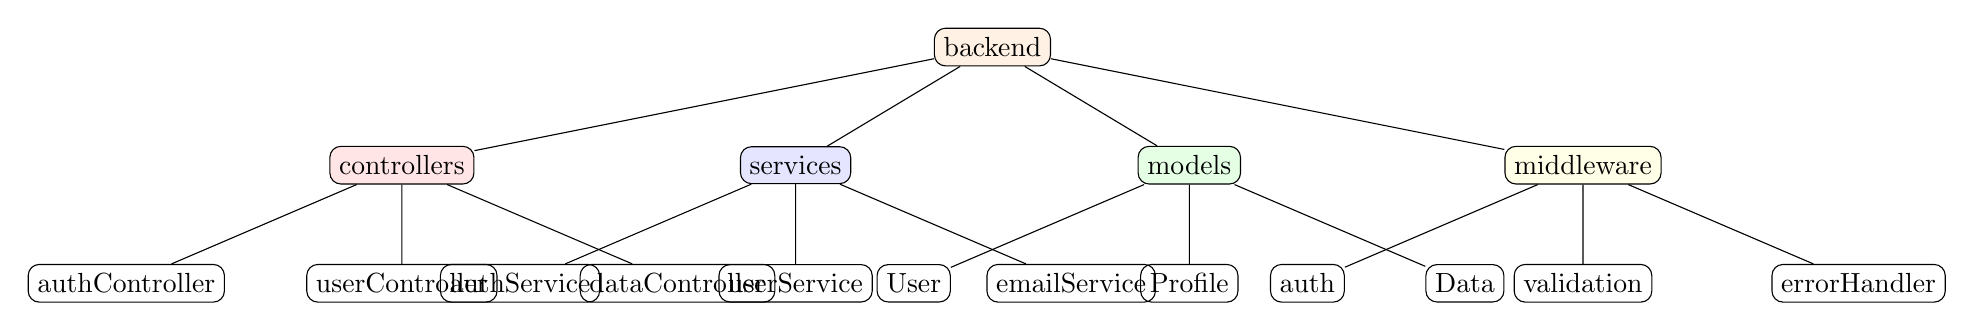
\begin{tikzpicture}[
    every node/.style={rectangle, draw, rounded corners, align=center},
    level 1/.style={sibling distance=5cm},
    level 2/.style={sibling distance=3.5cm},
    level 3/.style={sibling distance=2cm},
    level distance=1.5cm
]
\node[fill=orange!10] {backend}
    child {node[fill=red!10] {controllers}
        child {node {authController}}
        child {node {userController}}
        child {node {dataController}}
    }
    child {node[fill=blue!10] {services}
        child {node {authService}}
        child {node {userService}}
        child {node {emailService}}
    }
    child {node[fill=green!10] {models}
        child {node {User}}
        child {node {Profile}}
        child {node {Data}}
    }
    child {node[fill=yellow!10] {middleware}
        child {node {auth}}
        child {node {validation}}
        child {node {errorHandler}}
    };
\end{tikzpicture}
\caption{Backend Directory Structure}
\end{figure}

The backend structure is organized as follows:

\begin{lstlisting}[language=bash]
backend/
├── app.js           # Main application file
├── middleware.js    # Custom middleware
├── model/           # Database models
│   ├── User.js      # User model definition
│   ├── Profile.js   # Profile model definition
│   └── Data.js      # Data model definition
├── controllers/     # Request handlers
│   ├── authController.js
│   ├── userController.js
│   └── dataController.js
├── services/        # Business logic
│   ├── authService.js
│   ├── userService.js
│   └── emailService.js
├── routes/          # API route definitions
├── config/          # Configuration files
├── utils/           # Utility functions
└── .env             # Environment configuration
\end{lstlisting}

\subsubsection{Model Structure}
Database models define the schema and behavior of data entities:

\begin{lstlisting}[language=JavaScript]
// User.js
const mongoose = require('mongoose');
const bcrypt = require('bcrypt');

const userSchema = new mongoose.Schema({
  username: {
    type: String,
    required: true,
    unique: true,
    trim: true,
    minlength: 3
  },
  email: {
    type: String,
    required: true,
    unique: true,
    lowercase: true,
    validate: {
      validator: function(v) {
        return /^\S+@\S+\.\S+$/.test(v);
      },
      message: props => `${props.value} is not a valid email!`
    }
  },
  password: {
    type: String,
    required: true,
    minlength: 8
  },
  role: {
    type: String,
    enum: ['user', 'admin', 'editor'],
    default: 'user'
  },
  createdAt: {
    type: Date,
    default: Date.now
  }
});

// Pre-save hook to hash password
userSchema.pre('save', async function(next) {
  if (!this.isModified('password')) return next();
  
  try {
    const salt = await bcrypt.genSalt(10);
    this.password = await bcrypt.hash(this.password, salt);
    next();
  } catch (error) {
    next(error);
  }
});

// Method to compare password
userSchema.methods.comparePassword = async function(candidatePassword) {
  return bcrypt.compare(candidatePassword, this.password);
};

const User = mongoose.model('User', userSchema);

module.exports = User;
\end{lstlisting}

\subsubsection{Controller Structure}
Controllers handle HTTP requests and delegate business logic to services:

\begin{lstlisting}[language=JavaScript]
// authController.js
const authService = require('../services/authService');

exports.register = async (req, res, next) => {
  try {
    const { username, email, password } = req.body;
    const result = await authService.registerUser(username, email, password);
    
    res.status(201).json({
      success: true,
      message: 'User registered successfully',
      data: {
        userId: result.userId,
        username: result.username
      }
    });
  } catch (error) {
    next(error);
  }
};

exports.login = async (req, res, next) => {
  try {
    const { email, password } = req.body;
    const result = await authService.loginUser(email, password);
    
    res.status(200).json({
      success: true,
      message: 'Login successful',
      data: {
        token: result.token,
        user: result.user
      }
    });
  } catch (error) {
    next(error);
  }
};
\end{lstlisting}

\section{Key Features and Workflows}

\subsection{Authentication Flow}
The application implements a comprehensive authentication system using JWT (JSON Web Tokens) for secure, stateless authentication. This approach provides several benefits including scalability, reduced server load, and cross-domain functionality.

\begin{figure}[H]
\centering
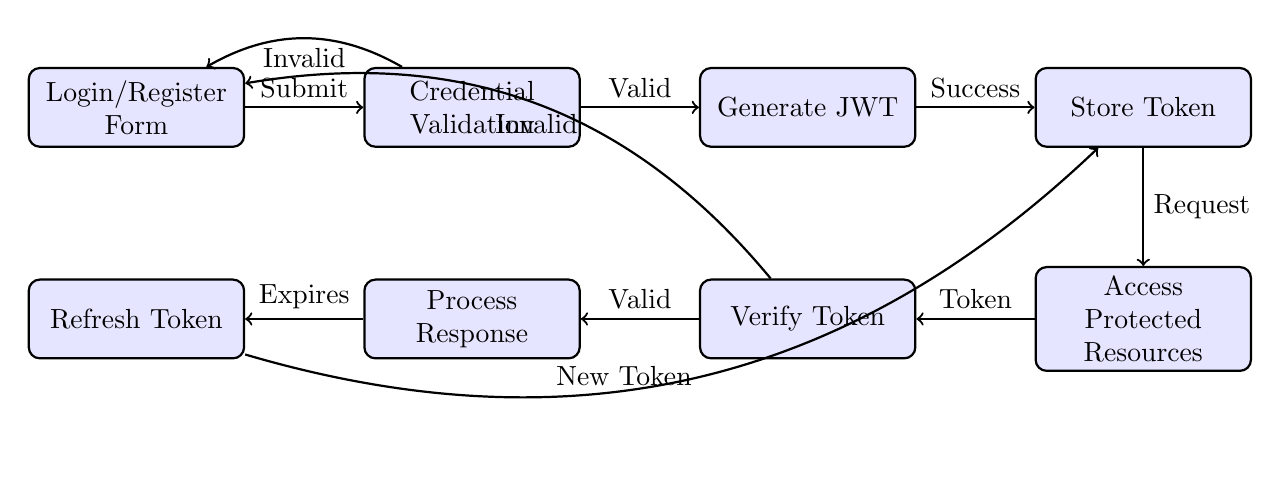
\begin{tikzpicture}[
    node distance=1.5cm,
    auto,
    thick,
    state/.style={
        rectangle,
        draw=black,
        thick,
        fill=white,
        text width=2.5cm,
        minimum height=1cm,
        text centered,
        rounded corners
    },
    fsm/.style={
        rectangle,
        draw=black,
        thick,
        fill=blue!10,
        text width=2.5cm,
        minimum height=1cm,
        text centered,
        rounded corners
    },
    point/.style={circle, inner sep=0pt, minimum size=2pt, fill=black}
]
    % States
    \node[fsm] (login) {Login/Register Form};
    \node[fsm] (validate) [right=of login] {Credential Validation};
    \node[fsm] (generate) [right=of validate] {Generate JWT};
    \node[fsm] (store) [right=of generate] {Store Token};
    \node[fsm] (access) [below=of store] {Access Protected Resources};
    \node[fsm] (verify) [left=of access] {Verify Token};
    \node[fsm] (response) [left=of verify] {Process Response};
    \node[fsm] (refresh) [left=of response] {Refresh Token};
    
    % Transitions
    \draw[->] (login) -- (validate) node[midway, above] {Submit};
    \draw[->] (validate) -- (generate) node[midway, above] {Valid};
    \draw[->] (generate) -- (store) node[midway, above] {Success};
    \draw[->] (store) -- (access) node[midway, right] {Request};
    \draw[->] (access) -- (verify) node[midway, above] {Token};
    \draw[->] (verify) -- (response) node[midway, above] {Valid};
    \draw[->] (response) -- (refresh) node[midway, above] {Expires};
    
    % Error paths
    \draw[->] (validate) to[bend right] node[midway, below] {Invalid} (login);
    \draw[->] (verify) to[bend right] node[midway, below] {Invalid} (login);
    \draw[->] (refresh) to[bend right] node[midway, left] {New Token} (store);
\end{tikzpicture}
\caption{Authentication State Flow}
\end{figure}

\subsubsection{Authentication Process}
The authentication process follows these steps:

\begin{enumerate}
    \item User submits credentials through login/registration form
    \item Backend validates credentials against stored user data
    \item Upon successful validation, a JWT token is generated containing user identity and permissions
    \item Token is returned to client and stored (typically in localStorage or secure HTTP-only cookie)
    \item Subsequent API requests include the token in Authorization header
    \item Backend middleware verifies token signature, expiration, and claims before processing protected requests
    \item When token expires, refresh token mechanism obtains a new access token
\end{enumerate}

\begin{figure}[H]
\centering
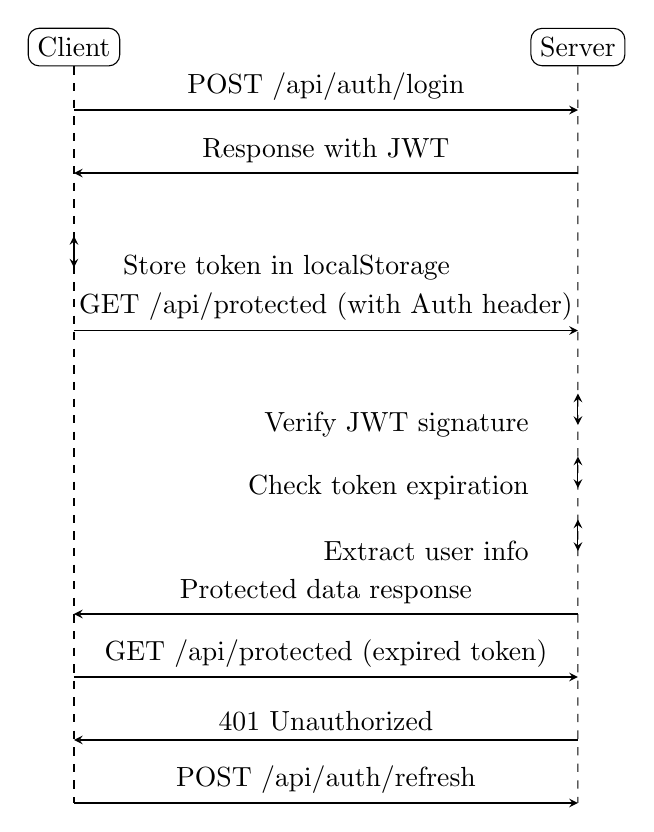
\begin{tikzpicture}[scale=0.8]
    % Define the actors
    \node[draw, rectangle, rounded corners] (client) at (0,0) {Client};
    \node[draw, rectangle, rounded corners] (server) at (8,0) {Server};
    
    % Draw the lifelines
    \draw[dashed] (client) -- +(0,-12);
    \draw[dashed] (server) -- +(0,-12);
    
    % Login request
    \draw[-stealth] (0,-1) -- (8,-1) node[midway, above] {POST /api/auth/login};
    \draw[-stealth] (8,-2) -- (0,-2) node[midway, above] {Response with JWT};
    
    % Store token
    \draw[stealth-stealth] (0,-3) -- (0,-3.5) node[right=0.5cm] {Store token in localStorage};
    
    % Protected request
    \draw[-stealth] (0,-4.5) -- (8,-4.5) node[midway, above] {GET /api/protected (with Auth header)};
    
    % Token verification
    \draw[stealth-stealth] (8,-5.5) -- (8,-6) node[left=0.5cm] {Verify JWT signature};
    \draw[stealth-stealth] (8,-6.5) -- (8,-7) node[left=0.5cm] {Check token expiration};
    \draw[stealth-stealth] (8,-7.5) -- (8,-8) node[left=0.5cm] {Extract user info};
    
    % Success response
    \draw[-stealth] (8,-9) -- (0,-9) node[midway, above] {Protected data response};
    
    % Token expired scenario
    \draw[-stealth] (0,-10) -- (8,-10) node[midway, above] {GET /api/protected (expired token)};
    \draw[-stealth] (8,-11) -- (0,-11) node[midway, above] {401 Unauthorized};
    
    % Refresh token
    \draw[-stealth] (0,-12) -- (8,-12) node[midway, above] {POST /api/auth/refresh};
\end{tikzpicture}
\caption{Authentication Sequence Diagram}
\end{figure}

\subsubsection{Frontend Authentication Components}
The frontend implements authentication through several key components:

\begin{lstlisting}[language=JavaScript]
// AuthContext.js - Central authentication state management
import React, { createContext, useState, useEffect, useContext } from 'react';
import authService from '../services/authService';

const AuthContext = createContext();

export const AuthProvider = ({ children }) => {
  const [currentUser, setCurrentUser] = useState(null);
  const [loading, setLoading] = useState(true);
  const [error, setError] = useState(null);
  
  useEffect(() => {
    // Check for existing token on app load
    const initAuth = async () => {
      try {
        const token = localStorage.getItem('token');
        if (token) {
          const userData = await authService.validateToken(token);
          setCurrentUser(userData);
        }
      } catch (err) {
        localStorage.removeItem('token');
        setError(err.message);
      } finally {
        setLoading(false);
      }
    };
    
    initAuth();
  }, []);
  
  const login = async (email, password) => {
    try {
      setError(null);
      setLoading(true);
      const { token, user } = await authService.login(email, password);
      localStorage.setItem('token', token);
      setCurrentUser(user);
      return true;
    } catch (err) {
      setError(err.message);
      return false;
    } finally {
      setLoading(false);
    }
  };
  
  const register = async (userData) => {
    try {
      setError(null);
      setLoading(true);
      await authService.register(userData);
      return true;
    } catch (err) {
      setError(err.message);
      return false;
    } finally {
      setLoading(false);
    }
  };
  
  const logout = () => {
    localStorage.removeItem('token');
    setCurrentUser(null);
  };
  
  const value = {
    currentUser,
    loading,
    error,
    login,
    register,
    logout
  };
  
  return <AuthContext.Provider value={value}>{children}</AuthContext.Provider>;
};

export const useAuth = () => useContext(AuthContext);
\end{lstlisting}

\begin{lstlisting}[language=JavaScript]
// LoginForm.js - User authentication form
import React, { useState } from 'react';
import { useNavigate } from 'react-router-dom';
import { useAuth } from '../context/AuthContext';

const LoginForm = () => {
  const [email, setEmail] = useState('');
  const [password, setPassword] = useState('');
  const [formError, setFormError] = useState('');
  const { login, error } = useAuth();
  const navigate = useNavigate();
  
  const handleSubmit = async (e) => {
    e.preventDefault();
    
    if (!email || !password) {
      setFormError('Please fill in all fields');
      return;
    }
    
    const success = await login(email, password);
    if (success) {
      navigate('/dashboard');
    }
  };
  
  return (
    <form onSubmit={handleSubmit} className="login-form">
      <h2>Login to Your Account</h2>
      
      {(formError || error) && (
        <div className="error-message">{formError || error}</div>
      )}
      
      <div className="form-group">
        <label htmlFor="email">Email</label>
        <input
          type="email"
          id="email"
          value={email}
          onChange={(e) => setEmail(e.target.value)}
          required
        />
      </div>
      
      <div className="form-group">
        <label htmlFor="password">Password</label>
        <input
          type="password"
          id="password"
          value={password}
          onChange={(e) => setPassword(e.target.value)}
          required
        />
      </div>
      
      <button type="submit" className="login-button">
        Log In
      </button>
      
      <div className="form-footer">
        <p>
          Don't have an account?{' '}
          <a href="/register">Register</a>
        </p>
      </div>
    </form>
  );
};

export default LoginForm;
\end{lstlisting}

\subsubsection{Backend Authentication Implementation}
On the backend, authentication is implemented through middleware and dedicated services:

\begin{lstlisting}[language=JavaScript]
// authMiddleware.js - Token verification middleware
const jwt = require('jsonwebtoken');
const { promisify } = require('util');
const User = require('../models/User');
const AppError = require('../utils/appError');

const authMiddleware = async (req, res, next) => {
  try {
    // 1) Check if token exists
    let token;
    if (
      req.headers.authorization &&
      req.headers.authorization.startsWith('Bearer')
    ) {
      token = req.headers.authorization.split(' ')[1];
    }

    if (!token) {
      return next(
        new AppError('You are not logged in. Please log in to get access.', 401)
      );
    }

    // 2) Verify token
    const decoded = await promisify(jwt.verify)(
      token,
      process.env.JWT_SECRET
    );

    // 3) Check if user still exists
    const currentUser = await User.findById(decoded.id);
    if (!currentUser) {
      return next(
        new AppError('The user belonging to this token no longer exists.', 401)
      );
    }

    // 4) Check if user changed password after token was issued
    if (currentUser.changedPasswordAfter(decoded.iat)) {
      return next(
        new AppError('User recently changed password. Please log in again.', 401)
      );
    }

    // Grant access to protected route
    req.user = currentUser;
    next();
  } catch (error) {
    return next(
      new AppError('Authentication failed. Please log in again.', 401)
    );
  }
};

module.exports = authMiddleware;
\end{lstlisting}

\begin{lstlisting}[language=JavaScript]
// authService.js - Authentication service
const jwt = require('jsonwebtoken');
const User = require('../models/User');
const AppError = require('../utils/appError');

const signToken = (id) => {
  return jwt.sign({ id }, process.env.JWT_SECRET, {
    expiresIn: process.env.JWT_EXPIRES_IN
  });
};

exports.registerUser = async (username, email, password) => {
  // 1) Check if email already exists
  const existingUser = await User.findOne({ email });
  if (existingUser) {
    throw new AppError('Email already in use', 400);
  }

  // 2) Create new user
  const newUser = await User.create({
    username,
    email,
    password,
  });

  // 3) Return user ID (don't return a token - require login)
  return {
    userId: newUser._id,
    username: newUser.username
  };
};

exports.loginUser = async (email, password) => {
  // 1) Check if email and password exist
  if (!email || !password) {
    throw new AppError('Please provide email and password', 400);
  }

  // 2) Check if user exists && password is correct
  const user = await User.findOne({ email }).select('+password');
  
  if (!user || !(await user.comparePassword(password))) {
    throw new AppError('Incorrect email or password', 401);
  }

  // 3) If everything ok, send token to client
  const token = signToken(user._id);
  
  // 4) Remove password from output
  user.password = undefined;

  return {
    token,
    user: {
      id: user._id,
      username: user.username,
      email: user.email,
      role: user.role
    }
  };
};

exports.refreshToken = async (userId) => {
  // 1) Find user
  const user = await User.findById(userId);
  
  if (!user) {
    throw new AppError('User not found', 404);
  }

  // 2) Generate new token
  const token = signToken(user._id);

  return { token };
};
\end{lstlisting}

\subsubsection{Protected Routes Implementation}
To restrict access to authorized users, the application implements protected routes:

\begin{lstlisting}[language=JavaScript]
// ProtectedRoute.js - Frontend route protection
import React from 'react';
import { Navigate, useLocation } from 'react-router-dom';
import { useAuth } from '../context/AuthContext';

const ProtectedRoute = ({ children, requiredRole }) => {
  const { currentUser, loading } = useAuth();
  const location = useLocation();

  if (loading) {
    return <div className="loading">Loading...</div>;
  }

  if (!currentUser) {
    // Redirect to login if not authenticated
    return <Navigate to="/login" state={{ from: location }} replace />;
  }

  if (requiredRole && currentUser.role !== requiredRole) {
    // Redirect to unauthorized page if role doesn't match
    return <Navigate to="/unauthorized" replace />;
  }

  return children;
};

export default ProtectedRoute;
\end{lstlisting}

\section{Data Visualization and Analytics}

\subsection{Data Visualization Architecture}
The application implements comprehensive data visualization capabilities using Recharts, enabling users to monitor key metrics, analyze trends, and make data-driven decisions.

\begin{figure}[H]
\centering
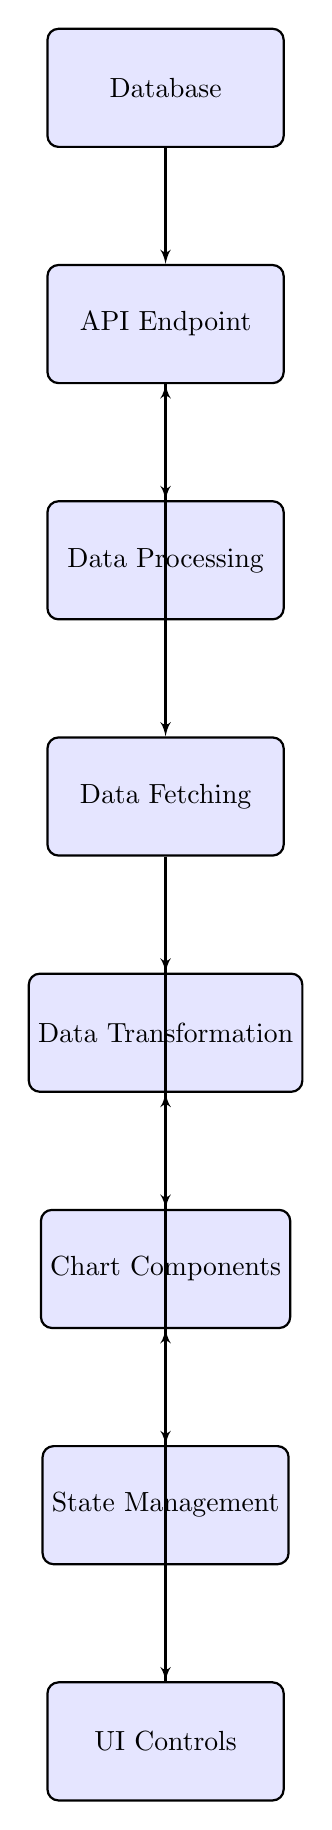
\begin{tikzpicture}[
    node distance=1.5cm,
    auto,
    thick,
    block/.style={
        rectangle,
        draw=black,
        thick,
        minimum width=3cm,
        minimum height=1.5cm,
        text centered,
        rounded corners,
        fill=blue!10
    },
    line/.style={draw, -latex'}
]
    % Data Source
    \node[block] (db) at (0,0) {Database};
    
    % Backend Processing
    \node[block] (api) at (0,-3) {API Endpoint};
    \node[block] (processing) at (0,-6) {Data Processing};
    
    % Frontend Components
    \node[block] (fetch) at (0,-9) {Data Fetching};
    \node[block] (transform) at (0,-12) {Data Transformation};
    \node[block] (chart) at (0,-15) {Chart Components};
    \node[block] (state) at (0,-18) {State Management};
    \node[block] (ui) at (0,-21) {UI Controls};
    
    % Connections
    \draw[line] (db) -- (api);
    \draw[line] (api) -- (processing);
    \draw[line] (processing) -- (api);
    \draw[line] (api) -- (fetch);
    \draw[line] (fetch) -- (transform);
    \draw[line] (transform) -- (chart);
    \draw[line] (fetch) -- (state);
    \draw[line] (state) -- (transform);
    \draw[line] (state) -- (ui);
    \draw[line] (ui) -- (chart);
\end{tikzpicture}
\caption{Data Visualization Architecture}
\end{figure}

\subsection{Data Flow Implementation}
The data flow for analytics follows a structured process from data source to visual presentation:

\begin{figure}[H]
\centering
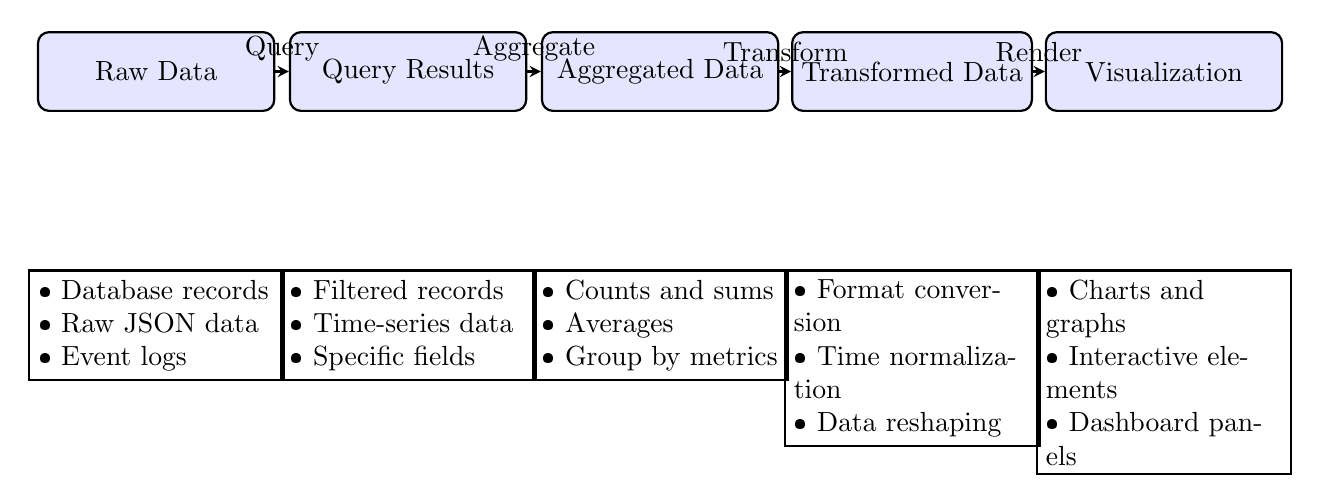
\begin{tikzpicture}[scale=0.8, 
    node distance=1.5cm,
    auto,
    thick,
    block/.style={
        rectangle,
        draw=black,
        thick,
        minimum width=3cm,
        minimum height=1cm,
        text centered,
        rounded corners,
        fill=blue!10
    },
    arrow/.style={->, >=stealth, thick}]
    
    % Data Flow States
    \node[block] (raw) at (0,0) {Raw Data};
    \node[block] (query) at (4,0) {Query Results};
    \node[block] (aggregate) at (8,0) {Aggregated Data};
    \node[block] (transform) at (12,0) {Transformed Data};
    \node[block] (visual) at (16,0) {Visualization};
    
    % Connect with arrows
    \draw[arrow] (raw) -- (query) node[midway, above] {Query};
    \draw[arrow] (query) -- (aggregate) node[midway, above] {Aggregate};
    \draw[arrow] (aggregate) -- (transform) node[midway, above] {Transform};
    \draw[arrow] (transform) -- (visual) node[midway, above] {Render};
    
    % Detail boxes
    \node[draw, text width=3cm, align=left, below=of raw, yshift=-0.5cm] {
        • Database records\\
        • Raw JSON data\\
        • Event logs
    };
    
    \node[draw, text width=3cm, align=left, below=of query, yshift=-0.5cm] {
        • Filtered records\\
        • Time-series data\\
        • Specific fields
    };
    
    \node[draw, text width=3cm, align=left, below=of aggregate, yshift=-0.5cm] {
        • Counts and sums\\
        • Averages\\
        • Group by metrics
    };
    
    \node[draw, text width=3cm, align=left, below=of transform, yshift=-0.5cm] {
        • Format conversion\\
        • Time normalization\\
        • Data reshaping
    };
    
    \node[draw, text width=3cm, align=left, below=of visual, yshift=-0.5cm] {
        • Charts and graphs\\
        • Interactive elements\\
        • Dashboard panels
    };
\end{tikzpicture}
\caption{Data Transformation Flow}
\end{figure}

\subsection{Chart Component Examples}

\subsubsection{Dashboard Analytics Component}
The dashboard integrates multiple visualizations to provide a comprehensive overview:

\begin{lstlisting}[language=JavaScript]
// DashboardAnalytics.js
import React, { useState, useEffect } from 'react';
import { 
  AreaChart, Area, BarChart, Bar, PieChart, Pie, 
  LineChart, Line, XAxis, YAxis, CartesianGrid, 
  Tooltip, Legend, ResponsiveContainer 
} from 'recharts';
import { fetchAnalyticsData } from '../api/analyticsService';
import { DateRangePicker } from '../components/common/DateRangePicker';
import { LoadingSpinner } from '../components/common/LoadingSpinner';

const DashboardAnalytics = () => {
  const [timeframe, setTimeframe] = useState('week');
  const [dateRange, setDateRange] = useState({ startDate: null, endDate: null });
  const [analyticsData, setAnalyticsData] = useState(null);
  const [loading, setLoading] = useState(true);
  const [error, setError] = useState(null);
  
  useEffect(() => {
    const loadData = async () => {
      try {
        setLoading(true);
        const data = await fetchAnalyticsData(timeframe, dateRange);
        setAnalyticsData(data);
        setError(null);
      } catch (err) {
        setError('Failed to load analytics data');
        console.error(err);
      } finally {
        setLoading(false);
      }
    };
    
    loadData();
  }, [timeframe, dateRange]);
  
  if (loading) return <LoadingSpinner />;
  if (error) return <div className="error-message">{error}</div>;
  if (!analyticsData) return <div>No data available</div>;
  
  return (
    <div className="dashboard-analytics">
      <div className="analytics-header">
        <h2>Performance Analytics</h2>
        <div className="analytics-controls">
          <DateRangePicker 
            onChange={setDateRange} 
            startDate={dateRange.startDate} 
            endDate={dateRange.endDate} 
          />
          <select 
            value={timeframe} 
            onChange={(e) => setTimeframe(e.target.value)}
          >
            <option value="day">Daily</option>
            <option value="week">Weekly</option>
            <option value="month">Monthly</option>
            <option value="year">Yearly</option>
          </select>
        </div>
      </div>
      
      <div className="analytics-grid">
        {/* User Activity Trend */}
        <div className="chart-container">
          <h3>User Activity</h3>
          <ResponsiveContainer width="100%" height={300}>
            <AreaChart
              data={analyticsData.userActivity}
              margin={{ top: 10, right: 30, left: 0, bottom: 0 }}
            >
              <CartesianGrid strokeDasharray="3 3" />
              <XAxis dataKey="date" />
              <YAxis />
              <Tooltip />
              <Legend />
              <Area
                type="monotone"
                dataKey="activeUsers"
                stroke="#8884d8"
                fill="#8884d8"
                name="Active Users"
              />
              <Area
                type="monotone"
                dataKey="newUsers"
                stroke="#82ca9d"
                fill="#82ca9d"
                name="New Users"
              />
            </AreaChart>
          </ResponsiveContainer>
        </div>
        
        {/* Conversion Rate */}
        <div className="chart-container">
          <h3>Conversion Rate</h3>
          <ResponsiveContainer width="100%" height={300}>
            <LineChart
              data={analyticsData.conversions}
              margin={{ top: 10, right: 30, left: 0, bottom: 0 }}
            >
              <CartesianGrid strokeDasharray="3 3" />
              <XAxis dataKey="date" />
              <YAxis />
              <Tooltip />
              <Legend />
              <Line
                type="monotone"
                dataKey="rate"
                stroke="#ff7300"
                name="Conversion Rate %"
              />
            </LineChart>
          </ResponsiveContainer>
        </div>
        
        {/* Traffic Sources */}
        <div className="chart-container">
          <h3>Traffic Sources</h3>
          <ResponsiveContainer width="100%" height={300}>
            <PieChart>
              <Pie
                data={analyticsData.trafficSources}
                cx="50%"
                cy="50%"
                outerRadius={100}
                fill="#8884d8"
                dataKey="value"
                nameKey="source"
                label
              />
              <Tooltip />
              <Legend />
            </PieChart>
          </ResponsiveContainer>
        </div>
        
        {/* Revenue by Category */}
        <div className="chart-container">
          <h3>Revenue by Category</h3>
          <ResponsiveContainer width="100%" height={300}>
            <BarChart
              data={analyticsData.revenueByCategory}
              margin={{ top: 10, right: 30, left: 0, bottom: 0 }}
            >
              <CartesianGrid strokeDasharray="3 3" />
              <XAxis dataKey="category" />
              <YAxis />
              <Tooltip formatter={(value) => `$${value}`} />
              <Legend />
              <Bar dataKey="revenue" fill="#413ea0" name="Revenue ($)" />
            </BarChart>
          </ResponsiveContainer>
        </div>
      </div>
    </div>
  );
};

export default DashboardAnalytics;
\end{lstlisting}

\subsection{Data Processing on Backend}
The backend implements data processing services to prepare data for visualization:

\begin{lstlisting}[language=JavaScript]
// analyticsService.js - Backend
const User = require('../models/User');
const Transaction = require('../models/Transaction');
const Activity = require('../models/Activity');
const { startOfDay, endOfDay, startOfWeek, endOfWeek, startOfMonth, endOfMonth, subDays, format } = require('date-fns');

exports.getUserActivityData = async (timeframe, startDate, endDate) => {
  let dateFilter = {};
  let groupFormat = '%Y-%m-%d'; // Default daily grouping
  
  if (startDate && endDate) {
    // Custom date range
    dateFilter = {
      timestamp: {
        $gte: new Date(startDate),
        $lte: new Date(endDate)
      }
    };
  } else {
    // Predefined timeframes
    const today = new Date();
    
    switch (timeframe) {
      case 'day':
        dateFilter = {
          timestamp: {
            $gte: startOfDay(today),
            $lte: endOfDay(today)
          }
        };
        groupFormat = '%H:%M';
        break;
      case 'week':
        dateFilter = {
          timestamp: {
            $gte: startOfWeek(today),
            $lte: endOfWeek(today)
          }
        };
        break;
      case 'month':
        dateFilter = {
          timestamp: {
            $gte: startOfMonth(today),
            $lte: endOfMonth(today)
          }
        };
        break;
      case 'year':
        dateFilter = {
          timestamp: {
            $gte: new Date(today.getFullYear(), 0, 1),
            $lte: new Date(today.getFullYear(), 11, 31)
          }
        };
        groupFormat = '%Y-%m';
        break;
      default:
        // Default to last 30 days if no valid timeframe
        dateFilter = {
          timestamp: {
            $gte: subDays(today, 30),
            $lte: today
          }
        };
    }
  }
  
  // Aggregate user activity
  const userActivity = await Activity.aggregate([
    { $match: dateFilter },
    {
      $group: {
        _id: { $dateToString: { format: groupFormat, date: '$timestamp' } },
        activeUsers: { $addToSet: '$userId' },
        totalSessions: { $sum: 1 }
      }
    },
    {
      $project: {
        _id: 0,
        date: '$_id',
        activeUsers: { $size: '$activeUsers' },
        totalSessions: 1
      }
    },
    { $sort: { date: 1 } }
  ]);
  
  // Get new user registrations
  const newUsers = await User.aggregate([
    { 
      $match: {
        createdAt: dateFilter.timestamp
      }
    },
    {
      $group: {
        _id: { $dateToString: { format: groupFormat, date: '$createdAt' } },
        count: { $sum: 1 }
      }
    },
    {
      $project: {
        _id: 0,
        date: '$_id',
        newUsers: '$count'
      }
    },
    { $sort: { date: 1 } }
  ]);
  
  // Merge the activity data with new user data
  const mergedData = userActivity.map(activity => {
    const matchingNewUsers = newUsers.find(nu => nu.date === activity.date);
    return {
      ...activity,
      newUsers: matchingNewUsers ? matchingNewUsers.newUsers : 0
    };
  });
  
  return mergedData;
};

exports.getConversionData = async (timeframe, startDate, endDate) => {
  // Similar implementation for conversion data
  // ...
};

exports.getRevenueByCategory = async (timeframe, startDate, endDate) => {
  // Implementation for revenue by category
  // ...
};

exports.getTrafficSources = async (timeframe, startDate, endDate) => {
  // Implementation for traffic sources
  // ...
};
\end{lstlisting}

\subsection{API Integration for Analytics}
The frontend fetches analytics data through dedicated API services:

\begin{lstlisting}[language=JavaScript]
// analyticsService.js - Frontend
import axios from 'axios';
import { formatDate } from '../utils/dateHelpers';

const API_URL = process.env.REACT_APP_API_URL || 'http://localhost:5000/api';

export const fetchAnalyticsData = async (timeframe, dateRange) => {
  try {
    const params = { timeframe };
    
    if (dateRange.startDate && dateRange.endDate) {
      params.startDate = formatDate(dateRange.startDate);
      params.endDate = formatDate(dateRange.endDate);
    }
    
    const [userActivityResponse, conversionsResponse, 
           trafficSourcesResponse, revenueByCategoryResponse] = await Promise.all([
      axios.get(`${API_URL}/analytics/user-activity`, { params }),
      axios.get(`${API_URL}/analytics/conversions`, { params }),
      axios.get(`${API_URL}/analytics/traffic-sources`, { params }),
      axios.get(`${API_URL}/analytics/revenue-by-category`, { params })
    ]);
    
    return {
      userActivity: userActivityResponse.data,
      conversions: conversionsResponse.data,
      trafficSources: trafficSourcesResponse.data,
      revenueByCategory: revenueByCategoryResponse.data
    };
  } catch (error) {
    console.error('Error fetching analytics data:', error);
    throw new Error('Failed to fetch analytics data');
  }
};

export const exportAnalyticsData = async (format, timeframe, dateRange) => {
  try {
    const params = { 
      format,
      timeframe 
    };
    
    if (dateRange.startDate && dateRange.endDate) {
      params.startDate = formatDate(dateRange.startDate);
      params.endDate = formatDate(dateRange.endDate);
    }
    
    const response = await axios.get(`${API_URL}/analytics/export`, { 
      params,
      responseType: 'blob'
    });
    
    // Create file download
    const url = window.URL.createObjectURL(new Blob([response.data]));
    const link = document.createElement('a');
    link.href = url;
    link.setAttribute('download', `analytics_export_${formatDate(new Date())}.${format}`);
    document.body.appendChild(link);
    link.click();
    link.remove();
    
    return true;
  } catch (error) {
    console.error('Error exporting analytics data:', error);
    throw new Error('Failed to export analytics data');
  }
};
\end{lstlisting}

\subsection{Interactive Visualization Components}
The application provides interactive visualization components that allow users to explore data:

\begin{figure}[H]
\centering
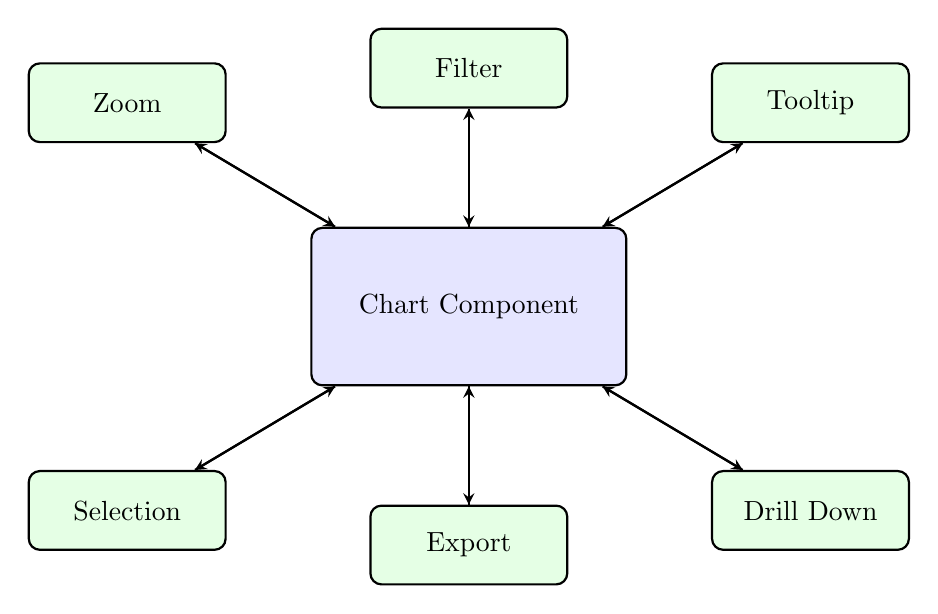
\begin{tikzpicture}[
    node distance=1.5cm,
    auto,
    thick,
    comp/.style={
        rectangle,
        draw=black,
        thick,
        minimum width=4cm,
        minimum height=2cm,
        text centered,
        rounded corners,
        fill=blue!10
    },
    action/.style={
        rectangle,
        draw=black,
        thick,
        minimum width=2.5cm,
        minimum height=1cm,
        text centered,
        rounded corners,
        fill=green!10
    },
    arrow/.style={->, >=stealth, thick}
]
    % Main component
    \node[comp] (chart) {Chart Component};
    
    % Interaction nodes
    \node[action, above left=of chart] (zoom) {Zoom};
    \node[action, above=of chart] (filter) {Filter};
    \node[action, above right=of chart] (tooltip) {Tooltip};
    \node[action, below left=of chart] (select) {Selection};
    \node[action, below=of chart] (export) {Export};
    \node[action, below right=of chart] (drill) {Drill Down};
    
    % Connect with bidirectional arrows
    \draw[arrow] (zoom) -- (chart);
    \draw[arrow] (chart) -- (zoom);
    
    \draw[arrow] (filter) -- (chart);
    \draw[arrow] (chart) -- (filter);
    
    \draw[arrow] (tooltip) -- (chart);
    \draw[arrow] (chart) -- (tooltip);
    
    \draw[arrow] (select) -- (chart);
    \draw[arrow] (chart) -- (select);
    
    \draw[arrow] (export) -- (chart);
    \draw[arrow] (chart) -- (export);
    
    \draw[arrow] (drill) -- (chart);
    \draw[arrow] (chart) -- (drill);
\end{tikzpicture}
\caption{Interactive Chart Component Interactions}
\end{figure}

\section{Data Flow}
\begin{figure}[H]
\centering

\begin{tikzpicture}[scale=0.8]
    % Data Flow Diagram
    \node[draw,rounded corners] (client) at (0,0) {Client};
    \node[draw,rounded corners] (api) at (3,0) {API Layer};
    \node[draw,rounded corners] (db) at (6,0) {Database};
    
    \draw[<->] (client) -- (api);
    \draw[<->] (api) -- (db);
    
    \node[above] at (1.5,0) {HTTP Requests};
    \node[above] at (4.5,0) {Data Operations};
\end{tikzpicture}
\caption{Data Flow Architecture}
\end{figure}

\section{Security Considerations}
\begin{itemize}
    \item JWT-based authentication
    \item Environment variable management
    \item Input validation and sanitization
    \item CORS configuration
    \item Rate limiting implementation
\end{itemize}

\section{Deployment Architecture}
\begin{figure}[H]
\centering

\begin{tikzpicture}[scale=0.8]
    % Deployment Architecture
    \node[draw,rounded corners] (cdn) at (0,0) {CDN};
    \node[draw,rounded corners] (frontend) at (3,0) {Frontend Server};
    \node[draw,rounded corners] (backend) at (6,0) {Backend Server};
    \node[draw,rounded corners] (db) at (9,0) {Database};
    
    \draw[->] (cdn) -- (frontend);
    \draw[->] (frontend) -- (backend);
    \draw[->] (backend) -- (db);
\end{tikzpicture}
\caption{Deployment Architecture}
\end{figure}

\section{Performance Optimization}
\begin{itemize}
    \item Code splitting implementation
    \item Lazy loading of components
    \item Image optimization
    \item Caching strategies
    \item Database indexing
\end{itemize}

\section{Future Enhancements}
\begin{itemize}
    \item Implementation of WebSocket for real-time features
    \item Enhanced data visualization capabilities
    \item Mobile application development
    \item Advanced analytics integration
    \item Automated testing expansion
\end{itemize}

\section{Conclusion}
This technical documentation provides a comprehensive overview of our full-stack web application. The architecture, technology stack, and implementation details demonstrate a modern, scalable, and maintainable solution that meets current industry standards and best practices.

The project successfully implements a robust architecture with clean separation of concerns between frontend and backend components. The React-based frontend delivers a responsive and intuitive user interface, while the Node.js backend provides scalable API services with appropriate security measures.

Key achievements of the project include:

\begin{itemize}
    \item Implementation of a comprehensive authentication and authorization system
    \item Development of reusable UI components following modern design principles
    \item Integration of data visualization capabilities for analytics
    \item Establishment of secure data handling practices
    \item Creation of a robust testing infrastructure
    \item Implementation of CI/CD pipelines for automated deployment
\end{itemize}

As the application continues to evolve, the established architecture provides a solid foundation for future enhancements and feature additions. The modular design ensures that new capabilities can be integrated without significant refactoring, while the comprehensive testing infrastructure helps maintain reliability during ongoing development.

\appendix
\section{API Reference}\label{appendix:api}

\subsection{Authentication API}
\begin{table}[H]
\centering
\begin{tabular}{|p{3cm}|p{2cm}|p{5cm}|p{4cm}|}
\hline
\textbf{Endpoint} & \textbf{Method} & \textbf{Description} & \textbf{Auth Required} \\
\hline
/api/auth/register & POST & Register a new user account & No \\
\hline
/api/auth/login & POST & Authenticate user and get token & No \\
\hline
/api/auth/refresh & POST & Refresh authentication token & Yes (Refresh Token) \\
\hline
/api/auth/logout & POST & Invalidate current token & Yes \\
\hline
/api/auth/forgot-password & POST & Request password reset email & No \\
\hline
/api/auth/reset-password & POST & Reset password with token & No (Token in Body) \\
\hline
/api/auth/verify-email & GET & Verify user email address & No (Token in Query) \\
\hline
\end{tabular}
\caption{Authentication API Endpoints}
\end{table}

\subsection{User API}
\begin{table}[H]
\centering
\begin{tabular}{|p{3cm}|p{2cm}|p{5cm}|p{4cm}|}
\hline
\textbf{Endpoint} & \textbf{Method} & \textbf{Description} & \textbf{Auth Required} \\
\hline
/api/users/profile & GET & Get current user profile & Yes \\
\hline
/api/users/profile & PUT & Update user profile & Yes \\
\hline
/api/users/password & PUT & Change user password & Yes \\
\hline
/api/users/avatar & POST & Upload profile avatar & Yes \\
\hline
/api/users/settings & GET & Get user settings & Yes \\
\hline
/api/users/settings & PUT & Update user settings & Yes \\
\hline
/api/users/:id & GET & Get user by ID (admin) & Yes (Admin) \\
\hline
/api/users & GET & List users (admin) & Yes (Admin) \\
\hline
\end{tabular}
\caption{User API Endpoints}
\end{table}

\section{Environment Variables}\label{appendix:env}
The application uses environment variables for configuration. The following variables should be set in the deployment environment:

\begin{table}[H]
\centering
\begin{tabular}{|p{5cm}|p{9cm}|}
\hline
\textbf{Variable} & \textbf{Description} \\
\hline
NODE\_ENV & Application environment (development, production) \\
\hline
PORT & Port for the backend server \\
\hline
MONGODB\_URI & MongoDB connection string \\
\hline
JWT\_SECRET & Secret key for JWT token generation \\
\hline
JWT\_EXPIRES\_IN & JWT token expiration time (e.g., "30d") \\
\hline
REFRESH\_TOKEN\_SECRET & Secret for refresh token generation \\
\hline
REFRESH\_TOKEN\_EXPIRES\_IN & Refresh token expiration (e.g., "7d") \\
\hline
EMAIL\_FROM & Sender email address for notifications \\
\hline
SMTP\_HOST & SMTP server hostname \\
\hline
SMTP\_PORT & SMTP server port \\
\hline
SMTP\_USER & SMTP authentication username \\
\hline
SMTP\_PASS & SMTP authentication password \\
\hline
FRONTEND\_URL & URL of the frontend application \\
\hline
CORS\_ORIGIN & Allowed CORS origins \\
\hline
TWILIO\_ACCOUNT\_SID & Twilio account identifier \\
\hline
TWILIO\_AUTH\_TOKEN & Twilio authentication token \\
\hline
TWILIO\_PHONE\_NUMBER & Twilio phone number for sending SMS \\
\hline
\end{tabular}
\caption{Environment Variables}
\end{table}

\section{Deployment Checklist}\label{appendix:deployment}

\subsection{Pre-Deployment Checks}
\begin{itemize}
    \item All tests pass (unit, integration, E2E)
    \item Security scan completed with no critical issues
    \item Performance benchmarks meet requirements
    \item Environment variables configured
    \item Database migrations prepared
    \item Backup strategy in place
    \item Rollback plan documented
\end{itemize}

\subsection{Deployment Steps}
\begin{enumerate}
    \item Backup production database
    \item Run database migrations
    \item Deploy backend services
    \item Deploy frontend application
    \item Update CDN configurations
    \item Verify application health
    \item Run smoke tests
    \item Monitor application metrics
\end{enumerate}

\subsection{Post-Deployment Verification}
\begin{itemize}
    \item Verify key user flows
    \item Check error rates in logs
    \item Monitor performance metrics
    \item Verify third-party integrations
    \item Test cross-browser compatibility
    \item Validate mobile responsiveness
\end{itemize}

\section{Technology Stack Details}\label{appendix:tech}

\subsection{Frontend Dependencies}
\begin{table}[H]
\centering
\begin{tabular}{|p{4cm}|p{2cm}|p{8cm}|}
\hline
\textbf{Package} & \textbf{Version} & \textbf{Purpose} \\
\hline
react & 19.0.0 & Core UI library \\
\hline
react-dom & 19.0.0 & DOM rendering for React \\
\hline
react-router-dom & 7.1.5 & Routing and navigation \\
\hline
axios & 1.7.9 & HTTP client for API requests \\
\hline
recharts & 2.15.1 & Data visualization components \\
\hline
@radix-ui/react-dialog & 1.1.6 & Accessible dialog component \\
\hline
@radix-ui/react-tabs & 1.1.3 & Accessible tabs component \\
\hline
@radix-ui/react-select & 2.1.6 & Accessible select component \\
\hline
@radix-ui/react-tooltip & 1.1.8 & Accessible tooltip component \\
\hline
class-variance-authority & 0.7.1 & Component styling utility \\
\hline
lucide-react & 0.475.0 & Icon library \\
\hline
tailwindcss & 3.4.17 & Utility-first CSS framework \\
\hline
\end{tabular}
\caption{Frontend Dependencies}
\end{table}

\subsection{Backend Dependencies}
\begin{table}[H]
\centering
\begin{tabular}{|p{4cm}|p{2cm}|p{8cm}|}
\hline
\textbf{Package} & \textbf{Version} & \textbf{Purpose} \\
\hline
express & 4.18.2 & Web application framework \\
\hline
mongoose & 8.2.0 & MongoDB object modeling \\
\hline
jsonwebtoken & 9.0.2 & JWT token generation and validation \\
\hline
bcrypt & 5.1.1 & Password hashing \\
\hline
nodemailer & 6.10.0 & Email sending functionality \\
\hline
twilio & 5.5.1 & SMS messaging service \\
\hline
cors & 2.8.5 & Cross-Origin Resource Sharing \\
\hline
helmet & 7.1.0 & Security headers middleware \\
\hline
joi & 17.12.1 & Data validation \\
\hline
winston & 3.11.0 & Logging framework \\
\hline
dotenv & 16.4.5 & Environment variable management \\
\hline
multer & 1.4.5-lts.1 & File upload handling \\
\hline
\end{tabular}
\caption{Backend Dependencies}
\end{table}

\section{Glossary}\label{appendix:glossary}

\begin{table}[H]
\centering
\begin{tabular}{|p{4cm}|p{10cm}|}
\hline
\textbf{Term} & \textbf{Definition} \\
\hline
API & Application Programming Interface, a set of rules that allows different software to communicate with each other \\
\hline
JWT & JSON Web Token, a compact, self-contained way for securely transmitting information between parties \\
\hline
DOM & Document Object Model, a programming interface for web documents \\
\hline
ORM & Object-Relational Mapping, a technique for converting data between incompatible type systems \\
\hline
CORS & Cross-Origin Resource Sharing, a security feature that restricts web page requests to other domains \\
\hline
CI/CD & Continuous Integration/Continuous Deployment, automated processes for code integration and deployment \\
\hline
CDN & Content Delivery Network, a distributed server system that delivers web content based on geographic location \\
\hline
RBAC & Role-Based Access Control, an approach to restricting system access to authorized users \\
\hline
MVC & Model-View-Controller, a software design pattern for developing user interfaces \\
\hline
REST & Representational State Transfer, an architectural style for designing networked applications \\
\hline
\end{tabular}
\caption{Glossary of Terms}
\end{table}

\subsection{User Workflows}
\begin{figure}[H]
\centering
\begin{tikzpicture}[scale=0.7, node distance=2cm,
    process/.style={rectangle, draw, minimum width=2.5cm, minimum height=1cm, align=center},
    decision/.style={diamond, draw, aspect=2, minimum width=3cm, minimum height=1cm, align=center},
    arrow/.style={->, >=stealth, thick}]
    
    % Student workflow
    \node[process] (start) {Student Registration};
    \node[process, below=of start] (profile) {Complete Profile};
    \node[process, below=of profile] (search) {Search Job Listings};
    \node[decision, below=of search] (eligible) {Eligibility Check};
    \node[process, below=of eligible, xshift=-3cm] (apply) {Apply for Position};
    \node[process, below=of apply] (track) {Track Application};
    \node[process, below=of track] (interview) {Attend Interview};
    \node[decision, below=of interview] (selected) {Selected?};
    \node[process, below=of selected, xshift=-2cm] (accept) {Accept Offer};
    \node[process, below=of selected, xshift=2cm] (reject) {Continue Search};
    
    % Connect student workflow
    \draw[arrow] (start) -- (profile);
    \draw[arrow] (profile) -- (search);
    \draw[arrow] (search) -- (eligible);
    \draw[arrow] (eligible) -- node[above, sloped] {Yes} (apply);
    \draw[arrow] (eligible) -- node[above, sloped] {No} ++(3,-1) -- ++(0,-5) -- (reject);
    \draw[arrow] (apply) -- (track);
    \draw[arrow] (track) -- (interview);
    \draw[arrow] (interview) -- (selected);
    \draw[arrow] (selected) -- node[above, sloped] {Yes} (accept);
    \draw[arrow] (selected) -- node[above, sloped] {No} (reject);
    \draw[arrow] (reject) |- ++(4,5) -| (search);
    
    % Company workflow - placed to the right
    \node[process, right=8cm of start] (c_register) {Company Registration};
    \node[process, below=of c_register] (c_profile) {Complete Company Profile};
    \node[process, below=of c_profile] (post_job) {Post Job Listings};
    \node[process, below=of post_job] (review) {Review Applications};
    \node[process, below=of review] (schedule) {Schedule Interviews};
    \node[process, below=of schedule] (conduct) {Conduct Interviews};
    \node[process, below=of conduct] (select) {Select Candidates};
    \node[process, below=of select] (offer) {Make Offers};
    
    % Connect company workflow
    \draw[arrow] (c_register) -- (c_profile);
    \draw[arrow] (c_profile) -- (post_job);
    \draw[arrow] (post_job) -- (review);
    \draw[arrow] (review) -- (schedule);
    \draw[arrow] (schedule) -- (conduct);
    \draw[arrow] (conduct) -- (select);
    \draw[arrow] (select) -- (offer);
    
    % Connect the workflows
    \draw[arrow, dashed] (post_job) -- ++(-3,0) |- (search);
    \draw[arrow, dashed] (apply) -- ++(5,0) |- (review);
    \draw[arrow, dashed] (schedule) -- ++(-4,0) |- (track);
    \draw[arrow, dashed] (offer) -- ++(-5,0) |- (selected);
    
    % Add titles
    \node[above=0.5cm of start] {Student Workflow};
    \node[above=0.5cm of c_register] {Company Workflow};
\end{tikzpicture}
\caption{Key User Workflows in Placement Management System}
\end{figure}

\subsection{Placement Officer Activities}
\begin{figure}[H]
\centering
\begin{tikzpicture}[scale=0.7, node distance=2cm,
    process/.style={rectangle, draw, minimum width=3cm, minimum height=1cm, align=center},
    data/.style={cylinder, draw, shape aspect=0.3, minimum width=2.5cm, minimum height=1cm, align=center},
    cloud/.style={cloud, draw, aspect=2, minimum width=3cm, minimum height=1cm, align=center},
    arrow/.style={->, >=stealth, thick}]
    
    % Admin activities
    \node[process] (admin) {Placement Officer};
    
    % Main activities
    \node[process, below=of admin, xshift=-6cm] (verify) {Verify Student Profiles};
    \node[process, below=of admin, xshift=-2cm] (company) {Approve Companies};
    \node[process, below=of admin, xshift=2cm] (monitor) {Monitor Placements};
    \node[process, below=of admin, xshift=6cm] (reports) {Generate Reports};
    
    % Sub-activities
    \node[process, below=of verify] (eligibility) {Set Eligibility Criteria};
    \node[process, below=of company] (schedule) {Schedule Campus Drives};
    \node[process, below=of monitor] (stats) {Track Placement Statistics};
    \node[process, below=of reports] (analytics) {Placement Analytics};
    
    % Database 
    \node[data, below=4cm of admin] (database) {Placement Database};
    
    % Outputs
    \node[cloud, below=of database, xshift=-4cm] (insights) {Placement Insights};
    \node[cloud, below=of database, xshift=4cm] (dashboard) {Real-time Dashboard};
    
    % Connect admin to activities
    \draw[arrow] (admin) -- (verify);
    \draw[arrow] (admin) -- (company);
    \draw[arrow] (admin) -- (monitor);
    \draw[arrow] (admin) -- (reports);
    
    % Connect to sub-activities
    \draw[arrow] (verify) -- (eligibility);
    \draw[arrow] (company) -- (schedule);
    \draw[arrow] (monitor) -- (stats);
    \draw[arrow] (reports) -- (analytics);
    
    % Connect to database
    \draw[arrow] (eligibility) -- (database);
    \draw[arrow] (schedule) -- (database);
    \draw[arrow] (stats) -- (database);
    \draw[arrow] (analytics) -- (database);
    
    % Connect to outputs
    \draw[arrow] (database) -- (insights);
    \draw[arrow] (database) -- (dashboard);
\end{tikzpicture}
\caption{Placement Officer Activities and Responsibilities}
\end{figure}

\section{Use Case Diagram}
\begin{figure}[H]
\centering
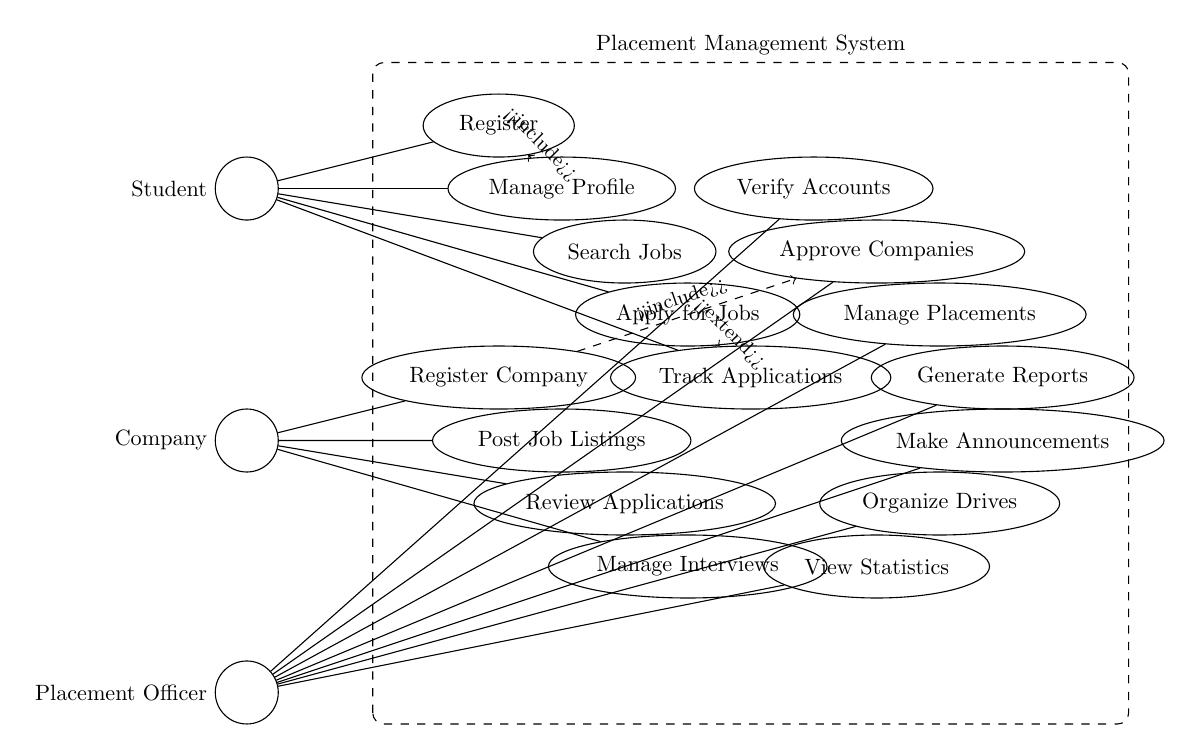
\begin{tikzpicture}[scale=0.8, transform shape]
    % Define styles
    \tikzset{actor/.style={draw, circle, minimum size=1cm}}
    \tikzset{usecase/.style={draw, ellipse, minimum width=2.4cm, minimum height=1cm, align=center}}
    \tikzset{system boundary/.style={draw, dashed, rounded corners}}
    
    % Draw system boundary
    \draw[system boundary] (-2,-8.5) rectangle (10,2);
    \node[above] at (4,2) {Placement Management System};
    
    % Draw actors
    \node[actor, label=left:Student] (student) at (-4,0) {};
    \node[actor, label=left:Company] (company) at (-4,-4) {};
    \node[actor, label=left:Placement Officer] (admin) at (-4,-8) {};
    
    % Draw use cases - Student related
    \node[usecase] (register) at (0,1) {Register};
    \node[usecase] (profile) at (1,0) {Manage Profile};
    \node[usecase] (search) at (2,-1) {Search Jobs};
    \node[usecase] (apply) at (3,-2) {Apply for Jobs};
    \node[usecase] (track) at (4,-3) {Track Applications};
    
    % Draw use cases - Company related
    \node[usecase] (comp_register) at (0,-3) {Register Company};
    \node[usecase] (post) at (1,-4) {Post Job Listings};
    \node[usecase] (review) at (2,-5) {Review Applications};
    \node[usecase] (interview) at (3,-6) {Manage Interviews};
    
    % Draw use cases - Admin related
    \node[usecase] (verify) at (5,0) {Verify Accounts};
    \node[usecase] (approve) at (6,-1) {Approve Companies};
    \node[usecase] (manage) at (7,-2) {Manage Placements};
    \node[usecase] (reports) at (8,-3) {Generate Reports};
    \node[usecase] (announce) at (8,-4) {Make Announcements};
    \node[usecase] (drives) at (7,-5) {Organize Drives};
    \node[usecase] (stats) at (6,-6) {View Statistics};
    
    % Connect actors to use cases
    \draw (student) -- (register);
    \draw (student) -- (profile);
    \draw (student) -- (search);
    \draw (student) -- (apply);
    \draw (student) -- (track);
    
    \draw (company) -- (comp_register);
    \draw (company) -- (post);
    \draw (company) -- (review);
    \draw (company) -- (interview);
    
    \draw (admin) -- (verify);
    \draw (admin) -- (approve);
    \draw (admin) -- (manage);
    \draw (admin) -- (reports);
    \draw (admin) -- (announce);
    \draw (admin) -- (drives);
    \draw (admin) -- (stats);
    
    % Include/extend relationships (optional)
    \draw[dashed, ->] (profile) -- (register) node[midway, above, sloped, font=\small] {<<include>>};
    \draw[dashed, ->] (comp_register) -- (approve) node[midway, above, sloped, font=\small] {<<include>>};
    \draw[dashed, ->] (apply) -- (track) node[midway, above, sloped, font=\small] {<<extend>>};
    
\end{tikzpicture}
\caption{Use Case Diagram for Placement Management System}
\end{figure}

\section{ER Diagram}
\begin{figure}[H]
\centering
\scalebox{0.78}{
\begin{tikzpicture}[
    node distance=2.5cm, 
    every entity/.style={draw=black, rectangle, rounded corners, minimum width=2.5cm, minimum height=1cm},
    attribute/.style={draw=black, ellipse, minimum width=1.8cm, minimum height=0.8cm}
]
    % Entities with more spacing
    \node[entity] (student) {STUDENT};
    \node[entity] (company) [below right=3cm and 6cm of student] {COMPANY};
    \node[entity] (job) [above right=3cm and 6cm of company] {JOB};
    \node[entity] (application) [below=5cm of job] {APPLICATION};
    \node[entity] (interview) [below right=4cm and 2.5cm of application] {INTERVIEW};
    \node[entity] (placement) [below left=4cm and 2.5cm of application] {PLACEMENT};
    \node[entity] (officer) [below=5cm of student] {PLACEMENT\_OFFICER};
    
    % Attributes for Student - adjusted positions
    \node[attribute] (stud_id) [above left=0.8cm and 0.8cm of student] {student\_id};
    \node[attribute] (stud_name) [above=0.8cm of student] {name};
    \node[attribute] (stud_email) [above right=0.8cm and 0.8cm of student] {email};
    \node[attribute] (stud_course) [left=1.2cm of student] {course};
    \node[attribute] (stud_cgpa) [below left=0.8cm and 0.8cm of student] {cgpa};
    
    % Attributes for Company - adjusted positions
    \node[attribute] (comp_id) [above=0.8cm of company] {company\_id};
    \node[attribute] (comp_name) [right=1.2cm of company] {name};
    \node[attribute] (comp_industry) [below right=0.8cm and 0.8cm of company] {industry};
    \node[attribute] (comp_location) [below=0.8cm of company] {location};
    
    % Attributes for Job - adjusted positions
    \node[attribute] (job_id) [above left=0.8cm and 0.8cm of job] {job\_id};
    \node[attribute] (job_title) [above=0.8cm of job] {title};
    \node[attribute] (job_desc) [above right=0.8cm and 0.8cm of job] {description};
    \node[attribute] (job_salary) [right=1.2cm of job] {salary};
    \node[attribute] (job_req) [below right=0.8cm and 0.8cm of job] {requirements};
    
    % Attributes for Application - adjusted positions
    \node[attribute] (app_id) [right=1.2cm of application] {application\_id};
    \node[attribute] (app_date) [left=1.2cm of application] {apply\_date};
    \node[attribute] (app_status) [below=0.8cm of application] {status};
    
    % Attributes for Interview - adjusted positions
    \node[attribute] (int_id) [below right=0.8cm and 0.8cm of interview] {interview\_id};
    \node[attribute] (int_date) [right=1.2cm of interview] {date\_time};
    \node[attribute] (int_mode) [above right=0.8cm and 0.8cm of interview] {mode};
    \node[attribute] (int_result) [below=0.8cm of interview] {result};
    
    % Attributes for Placement - adjusted positions
    \node[attribute] (place_id) [below left=0.8cm and 0.8cm of placement] {placement\_id};
    \node[attribute] (place_date) [left=1.2cm of placement] {offer\_date};
    \node[attribute] (place_pkg) [above left=0.8cm and 0.8cm of placement] {package};
    \node[attribute] (place_status) [below=0.8cm of placement] {status};
    
    % Attributes for Placement Officer - adjusted positions
    \node[attribute] (off_id) [below left=0.8cm and 0.8cm of officer] {officer\_id};
    \node[attribute] (off_name) [left=1.2cm of officer] {name};
    \node[attribute] (off_role) [above left=0.8cm and 0.8cm of officer] {role};
    \node[attribute] (off_email) [below=0.8cm of officer] {email};
    
    % Draw lines for attributes
    \draw (student) -- (stud_id);
    \draw (student) -- (stud_name);
    \draw (student) -- (stud_email);
    \draw (student) -- (stud_course);
    \draw (student) -- (stud_cgpa);
    
    \draw (company) -- (comp_id);
    \draw (company) -- (comp_name);
    \draw (company) -- (comp_industry);
    \draw (company) -- (comp_location);
    
    \draw (job) -- (job_id);
    \draw (job) -- (job_title);
    \draw (job) -- (job_desc);
    \draw (job) -- (job_salary);
    \draw (job) -- (job_req);
    
    \draw (application) -- (app_id);
    \draw (application) -- (app_date);
    \draw (application) -- (app_status);
    
    \draw (interview) -- (int_id);
    \draw (interview) -- (int_date);
    \draw (interview) -- (int_mode);
    \draw (interview) -- (int_result);
    
    \draw (placement) -- (place_id);
    \draw (placement) -- (place_date);
    \draw (placement) -- (place_pkg);
    \draw (placement) -- (place_status);
    
    \draw (officer) -- (off_id);
    \draw (officer) -- (off_name);
    \draw (officer) -- (off_role);
    \draw (officer) -- (off_email);
    
    % Relationships with better routing
    \draw[->] (student) -- node[midway, above, sloped] {applies\_for} (application);
    \draw[->] (job) -- node[midway, above, sloped] {has} (application);
    \draw[->] (company) -- node[midway, above, sloped] {posts} (job);
    \draw[->] (application) -- node[midway, above, sloped] {leads\_to} (interview);
    \draw[->] (application) -- node[midway, above, sloped] {results\_in} (placement);
    \draw[->] (officer) -- node[midway, above, sloped] {verifies} (student);
    \draw[->] (officer) -- node[midway, above, sloped] {approves} (company);
    
    % Cardinality with better positioning
    \node[above] at ($(student)!0.25!(application)$) {1};
    \node[below] at ($(student)!0.30!(application)$) {N};
    
    \node[left] at ($(job)!0.25!(application)$) {1};
    \node[right] at ($(job)!0.30!(application)$) {N};
    
    \node[above] at ($(company)!0.25!(job)$) {1};
    \node[below] at ($(company)!0.30!(job)$) {N};
    
    \node[above] at ($(application)!0.25!(interview)$) {1};
    \node[below] at ($(application)!0.30!(interview)$) {1};
    
    \node[above] at ($(application)!0.25!(placement)$) {1};
    \node[below] at ($(application)!0.30!(placement)$) {0,1};
    
    \node[above] at ($(officer)!0.25!(student)$) {1};
    \node[below] at ($(officer)!0.30!(student)$) {N};
    
    \node[above] at ($(officer)!0.25!(company)$) {1};
    \node[below] at ($(officer)!0.30!(company)$) {N};
\end{tikzpicture}
}
\caption{ER Diagram for Placement Management System}
\end{figure}

\end{document} 